\chapterimage{Pictures/chap08/dragons-fourier-600x1200.png}
\chapter{反射模型}\label{chap:反射模型}
\setcounter{sidenote}{1}
本章定义一组类来描述光在表面上散射的方式。回想\refsub{BRDF}中
我们介绍了双向反射分布函数(BRDF)抽象来描述表面的光反射,
双向透射分布函数(BTDF)来描述表面的透射,以及
双向散射分布函数(BSFD)来统合这两种效应。
本章中,我们将从为这些表面反射和透射函数定义通用接口开始。

许多来自表面的散射通常最好描述为多个BRDF和BTDF随空间变化的混合体;
在第\refchap{材质},我们将介绍结合了多个BRDF和BTDF的BSDF对象
以表示来自表面的整体散射。本章回避了反射和折射性质随表面变化的问题;
第\refchap{纹理}的纹理类将解决该问题。
BRDF和BTDF只显式建模了在表面上同一点入射和出射的光的散射。
对于展现出有意义的次表面光传输的曲面,我们将引入类\refvar{BSSRDF}{},
在第\refchap{体积散射}介绍一些相关理论后,它将在\refsec{BSSRDF}对次表面散射建模。

表面反射模型有以下几个来源:
\begin{itemize}
      \item \emph{测量的数据}:许多真实世界表面的反射分布性质已在实验室中测定。
            这样的数据可直接以表格形式使用或用来为一组基函数计算系数。
      \item \emph{现象模型}\sidenote{译者注:原文phenomenological models。}:
            试图描述真实世界表面定性性质的方程在仿真时可能很有效。
            这类BSDF可能很容易使用,因为它们常常有直观的参数来修改其表现(例如“粗糙度”)。
      \item \emph{模拟}:有时关于表面组成的底层信息是已知的。
            例如,我们可能知道涂料是悬浮在介质中的平均大小彩色颗粒组成的,
            或者某种布料是两种织线组成的,且知道每种的反射性质。
            在这些情况下,可以模拟来自微观几何体的光散射来生成反射数据。
            该模拟可在渲染时进行,或作为预处理完成后去适配一组基函数供渲染时使用。
      \item \emph{物理(波动)光学}:一些反射模型是用详细的光模型推导出的,
            将其视作波并计算麦克斯韦方程组的解以求解光是怎么从已知性质的表面散射的。
            这些模型常常计算量很大,然而对于渲染应用而言它们通常并不比基于几何光学的模型精确多少。
      \item \emph{几何光学}:像模拟方法那样,如果表面的底层散射和几何性质已知,
            则有时能直接从这些描述中推出解析式的反射模型。几何光学让建模光与表面的交互
            更加容易处理,因为可以忽略像偏振那样的复杂波动效应。
\end{itemize}
本章末的“扩展阅读”一节给出了许多这样的反射模型索引。

在我们定义相关接口前,简要回顾下它们是怎么嵌入整个系统的。
如果用了\refvar{SamplerIntegrator}{},则会为每条光线
调用方法\refvar[Li]{SamplerIntegrator::Li}{()}的实现。
在找到与几何图元最近的相交处后,它调用与该图元关联的表面着色器。
表面着色器实现为\refvar{Material}{}子类的方法并负责决定表面上特定点的BSDF是什么;
它返回的BSDF对象持有BRDF和BTDF且已分配内存和初始化来表示该点的散射。
然后积分器基于该点的入射光照用BSDF计算该点的散射光
(使用\refvar{BDPTIntegrator}{}、\refvar{MLTIntegrator}{}或\refvar{SPPMIntegrator}{}而
不是\refvar{SamplerIntegrator}{}的过程大致相同)。

\subsection{基本术语}\label{sub:基本术语}
为了能比较不同反射模型的视觉表现,我们将介绍一些基本术语以描述来自表面的反射。

来自表面的反射可分为四大类:\keyindex{漫反射}{diffuse}{}、\keyindex{光泽镜面}{glossy specular}{}、
\keyindex{完美镜面}{perfect specular}{}和\keyindex{逆反射}{retro-reflective}{}(\reffig{8.1})。
大多数真实表面展现的反射都是这四种的混合。漫反射表面在所有方向均等地散射光。
尽管完美的漫反射表面是不可物理实现的,但几乎是漫反射表面的例子包括暗沉的黑板和哑光的油漆。
光泽镜面表面例如塑料或高光泽涂料优先在一组反射方向上散射光——
它们展示了其他物体的模糊反射。完美镜像表面将入射光朝单个出射方向散射。
镜子和玻璃就是完美镜面表面的例子。
最后,像天鹅绒或月壤那样的逆反射表面主要沿着入射方向把光散射回去。
本章的图像将展示渲染场景中使用这几种反射的差别。
\begin{figure}[htbp]
      \centering
      \subfloat[漫反射BSDF]{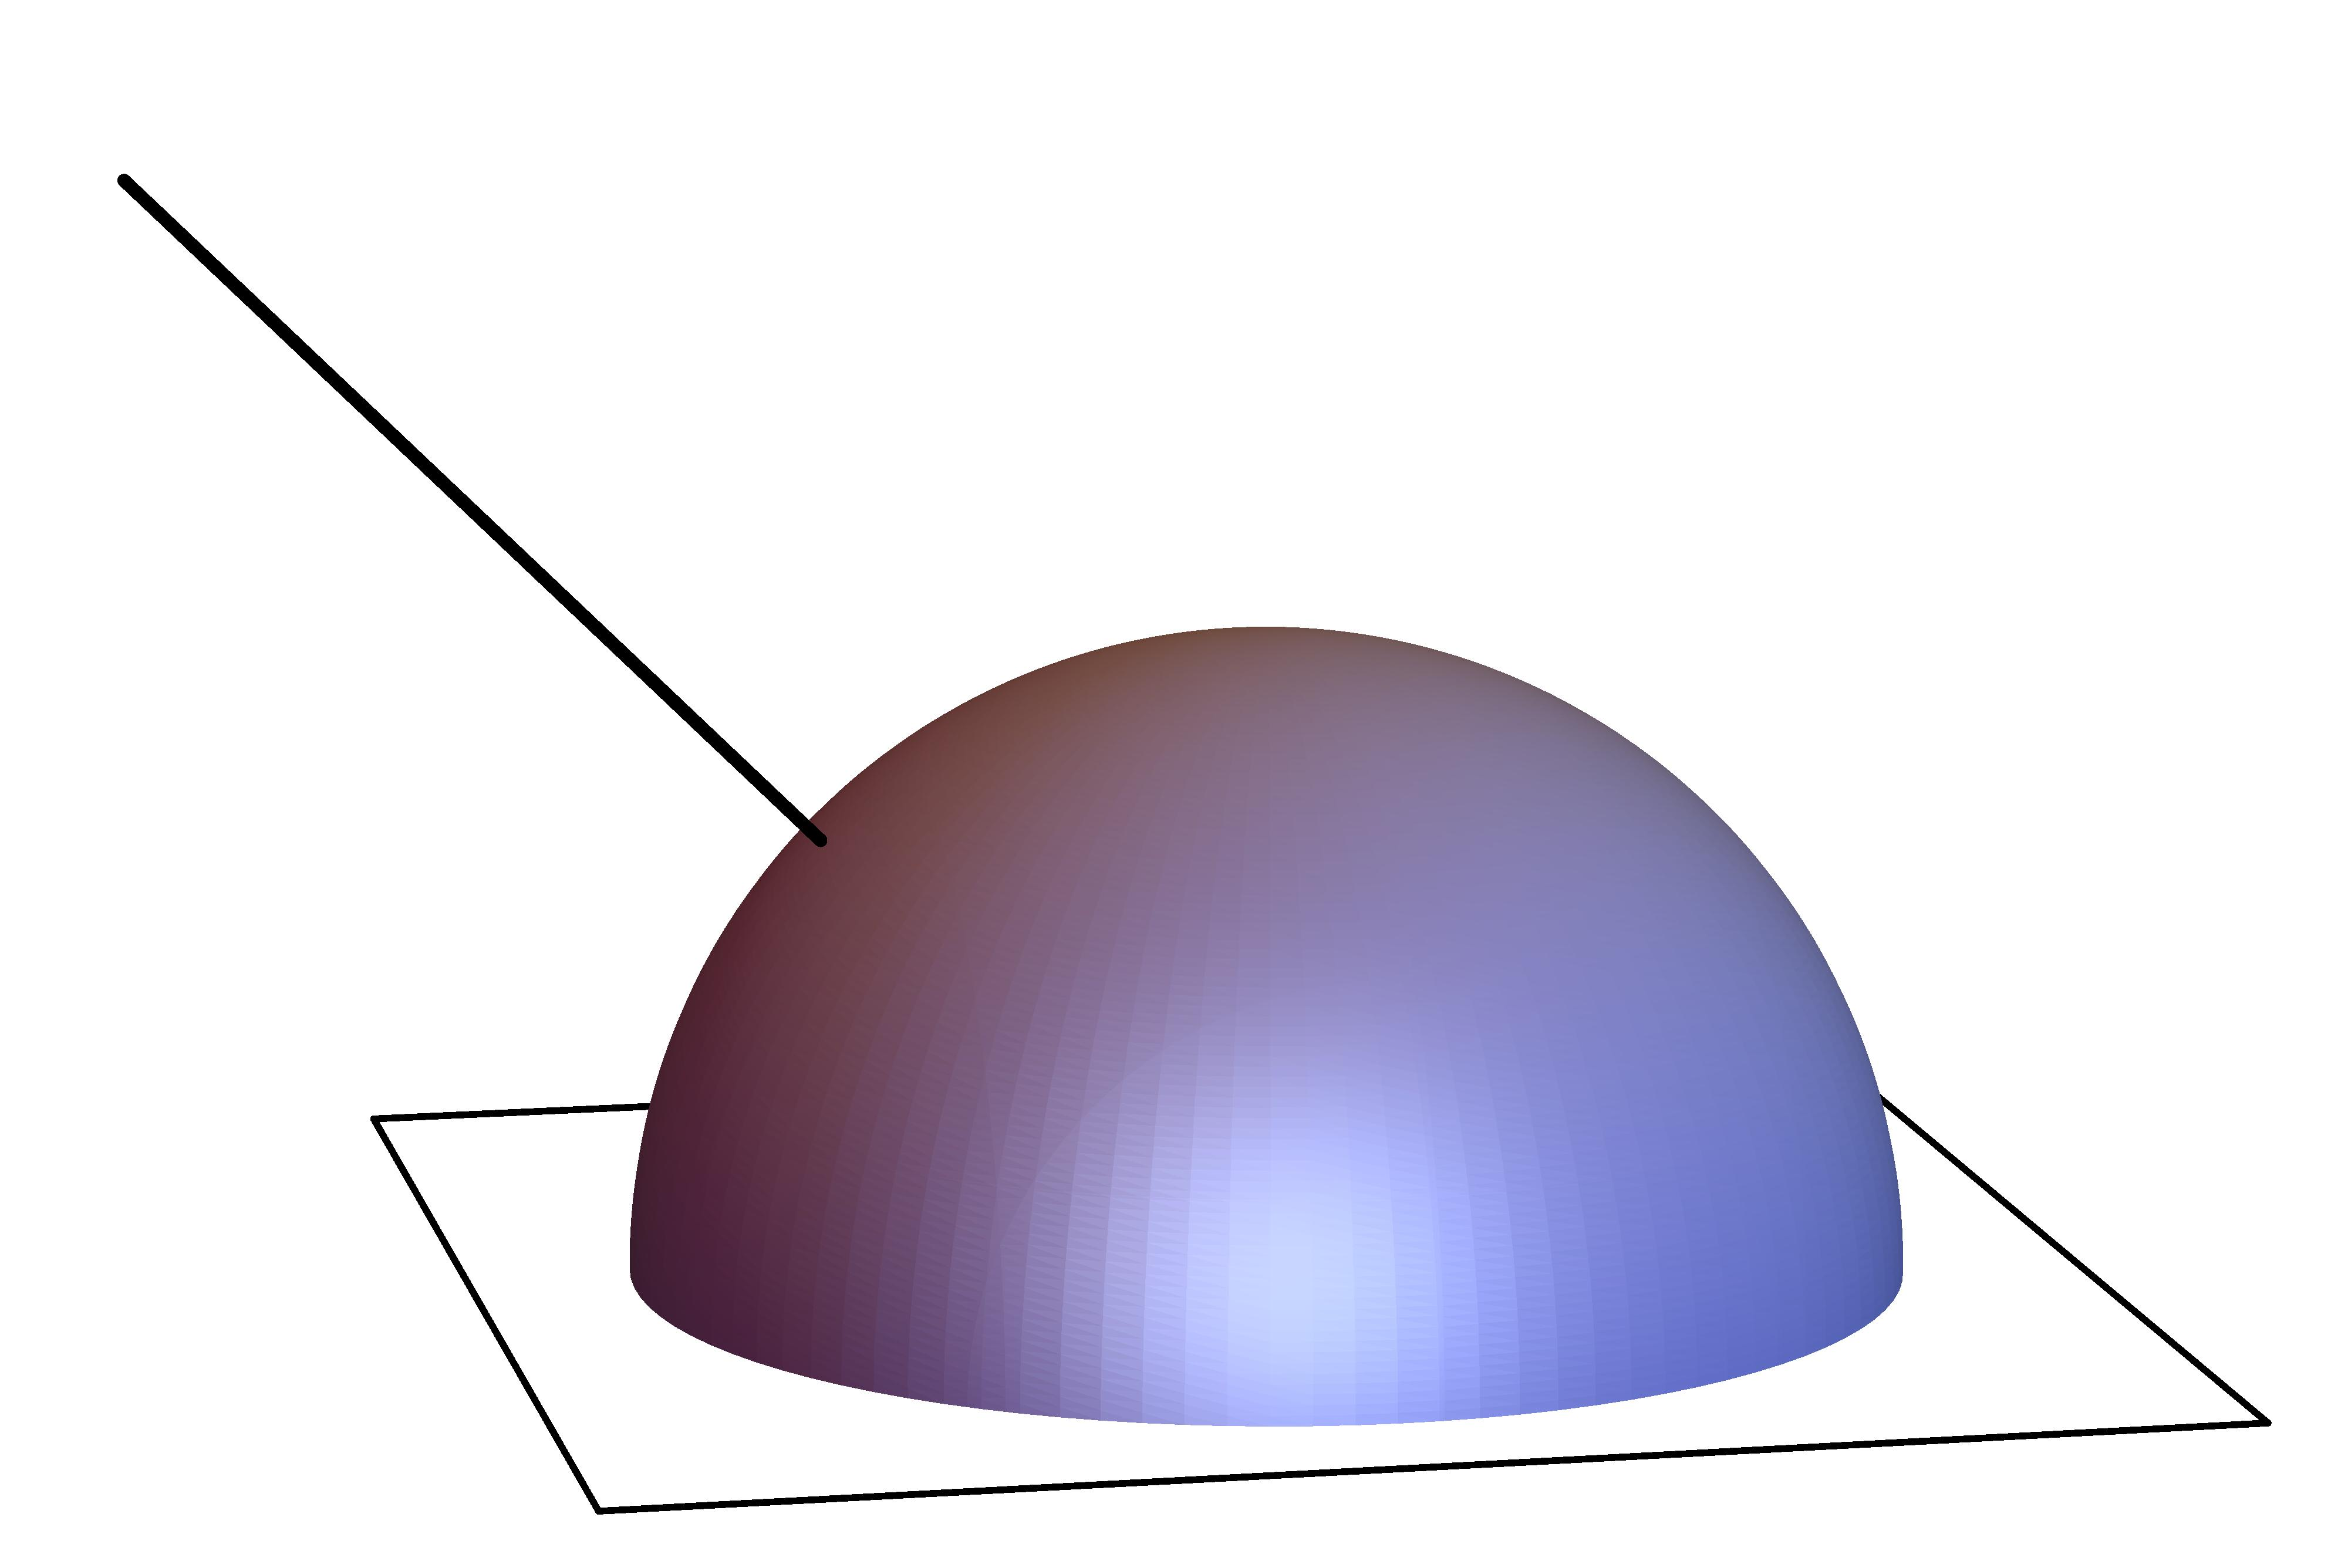
\includegraphics[width=0.5\linewidth]{chap08/brdf-diffuse-plot.jpg}\label{fig:8.1.1}}
      \subfloat[光泽BRDF]{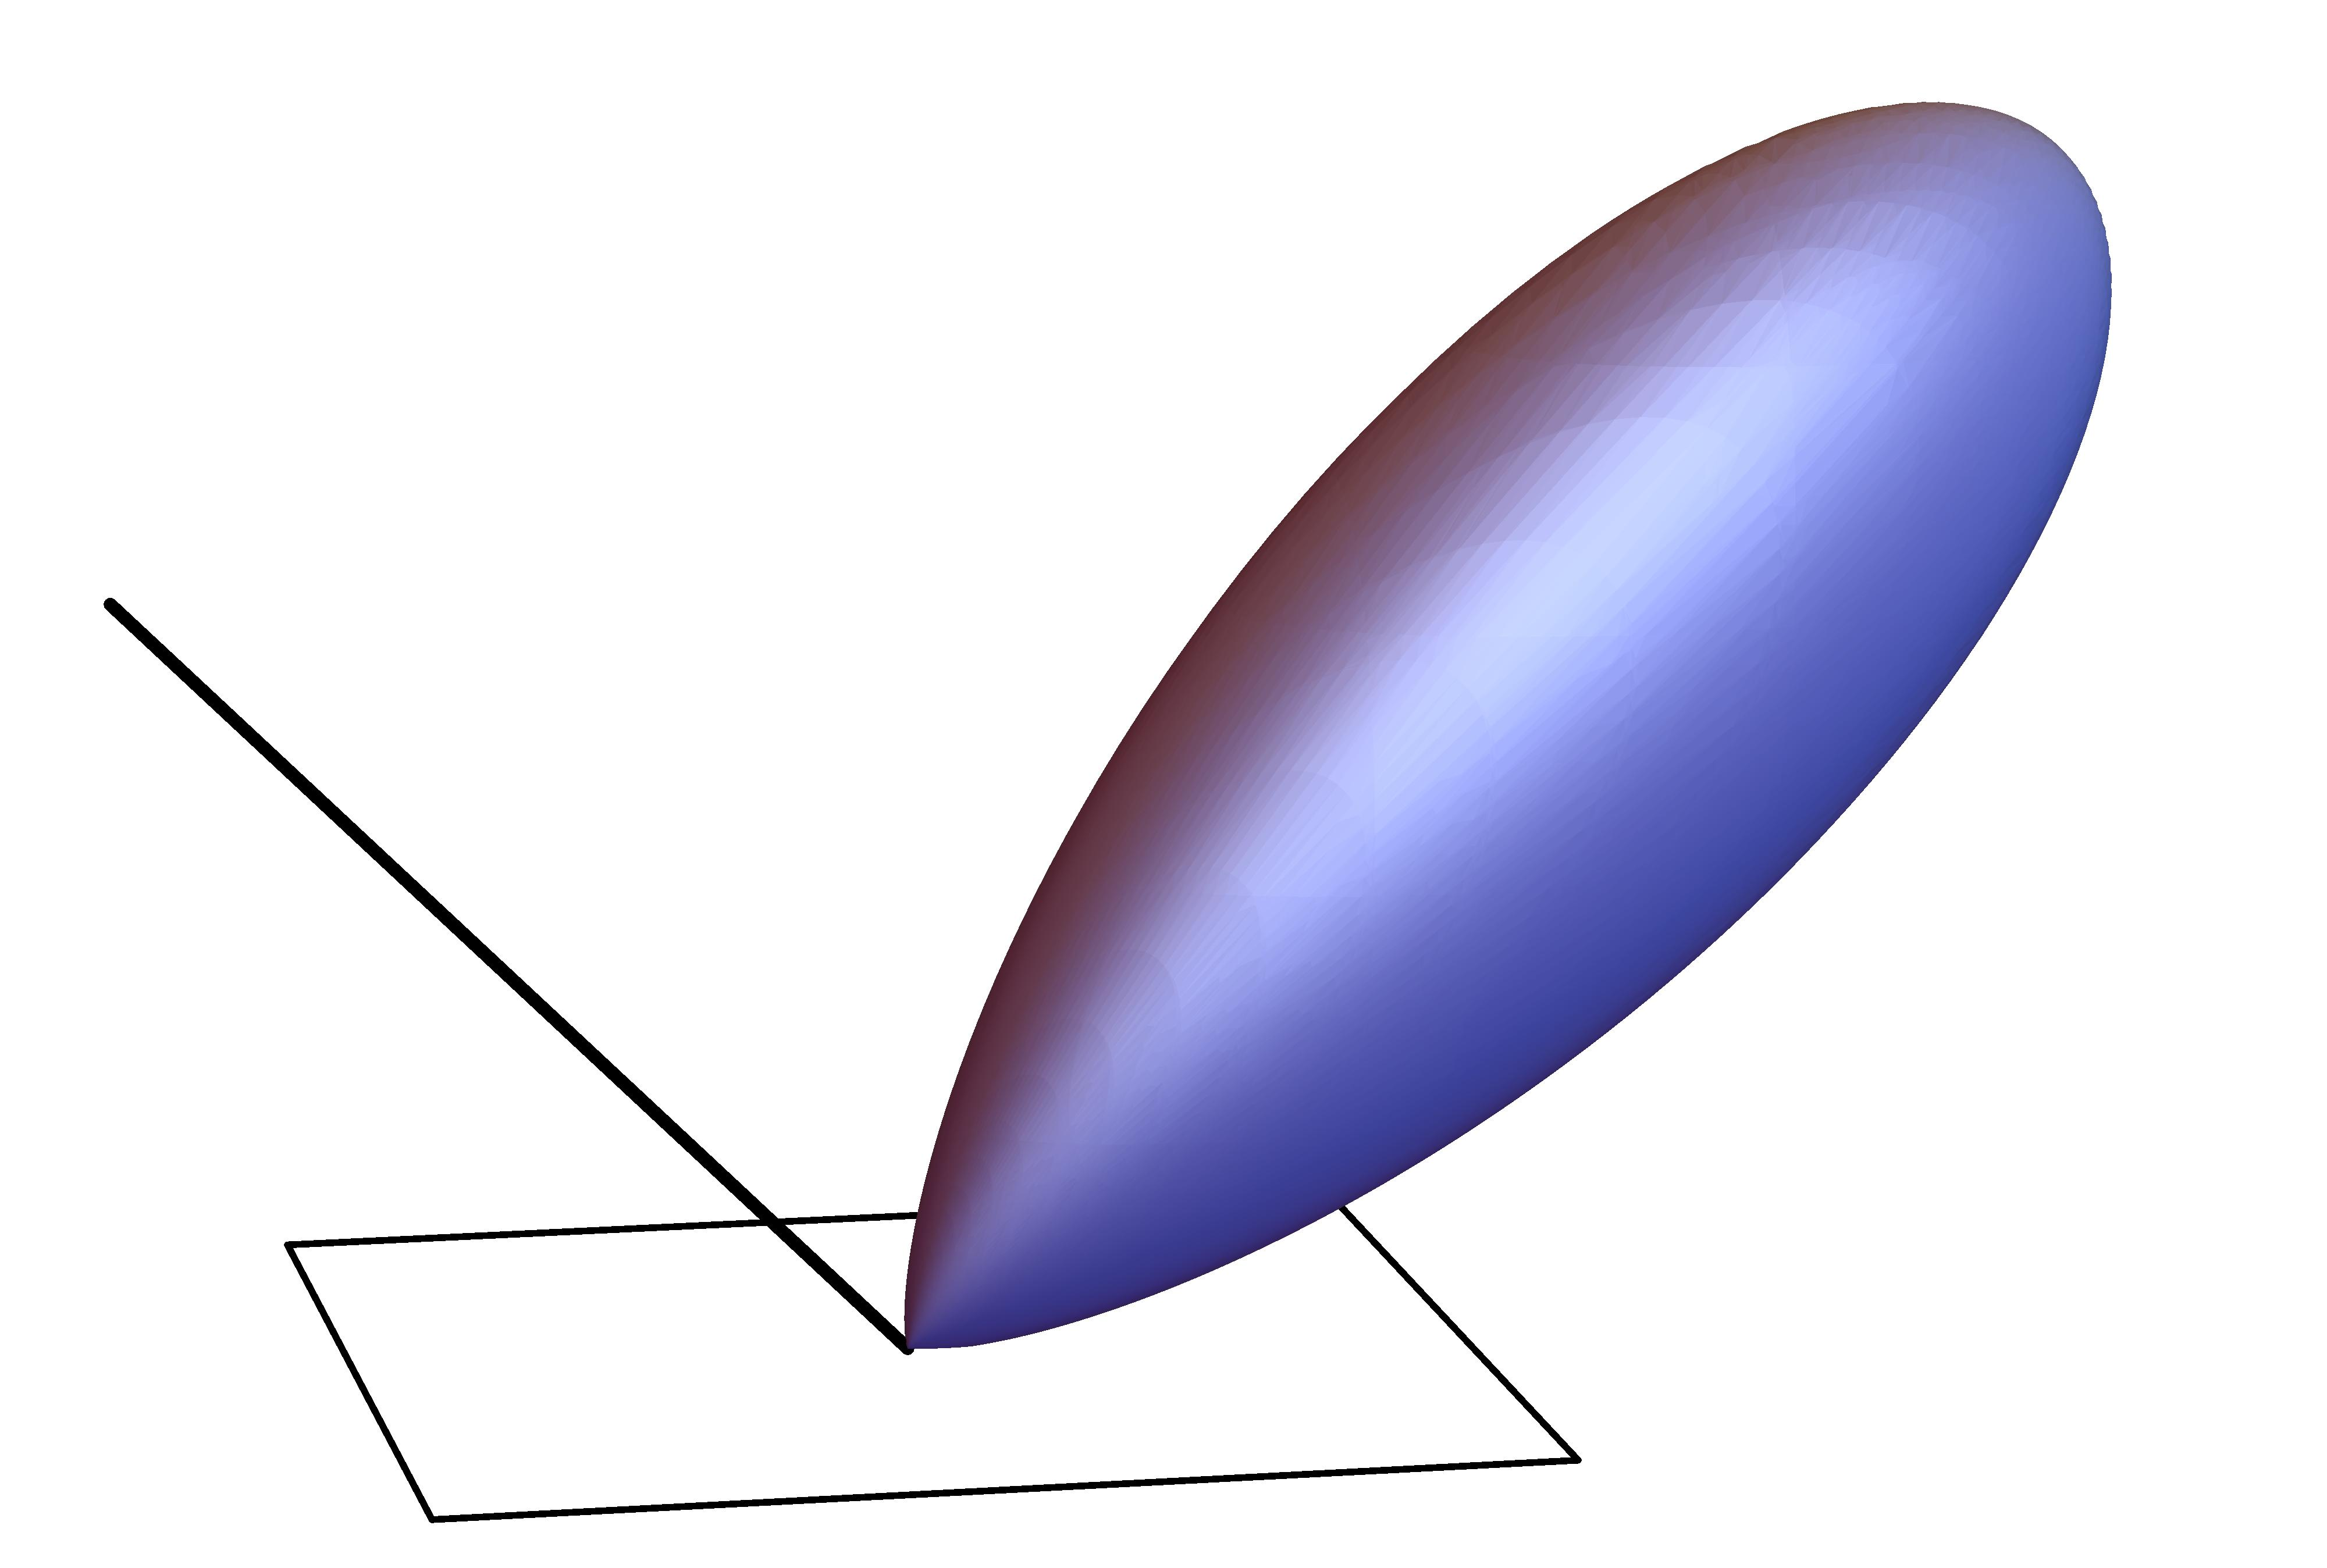
\includegraphics[width=0.5\linewidth]{chap08/brdf-glossy-plot.jpg}\label{fig:8.1.2}}\\
      \subfloat[几乎完美的镜面BRDF]{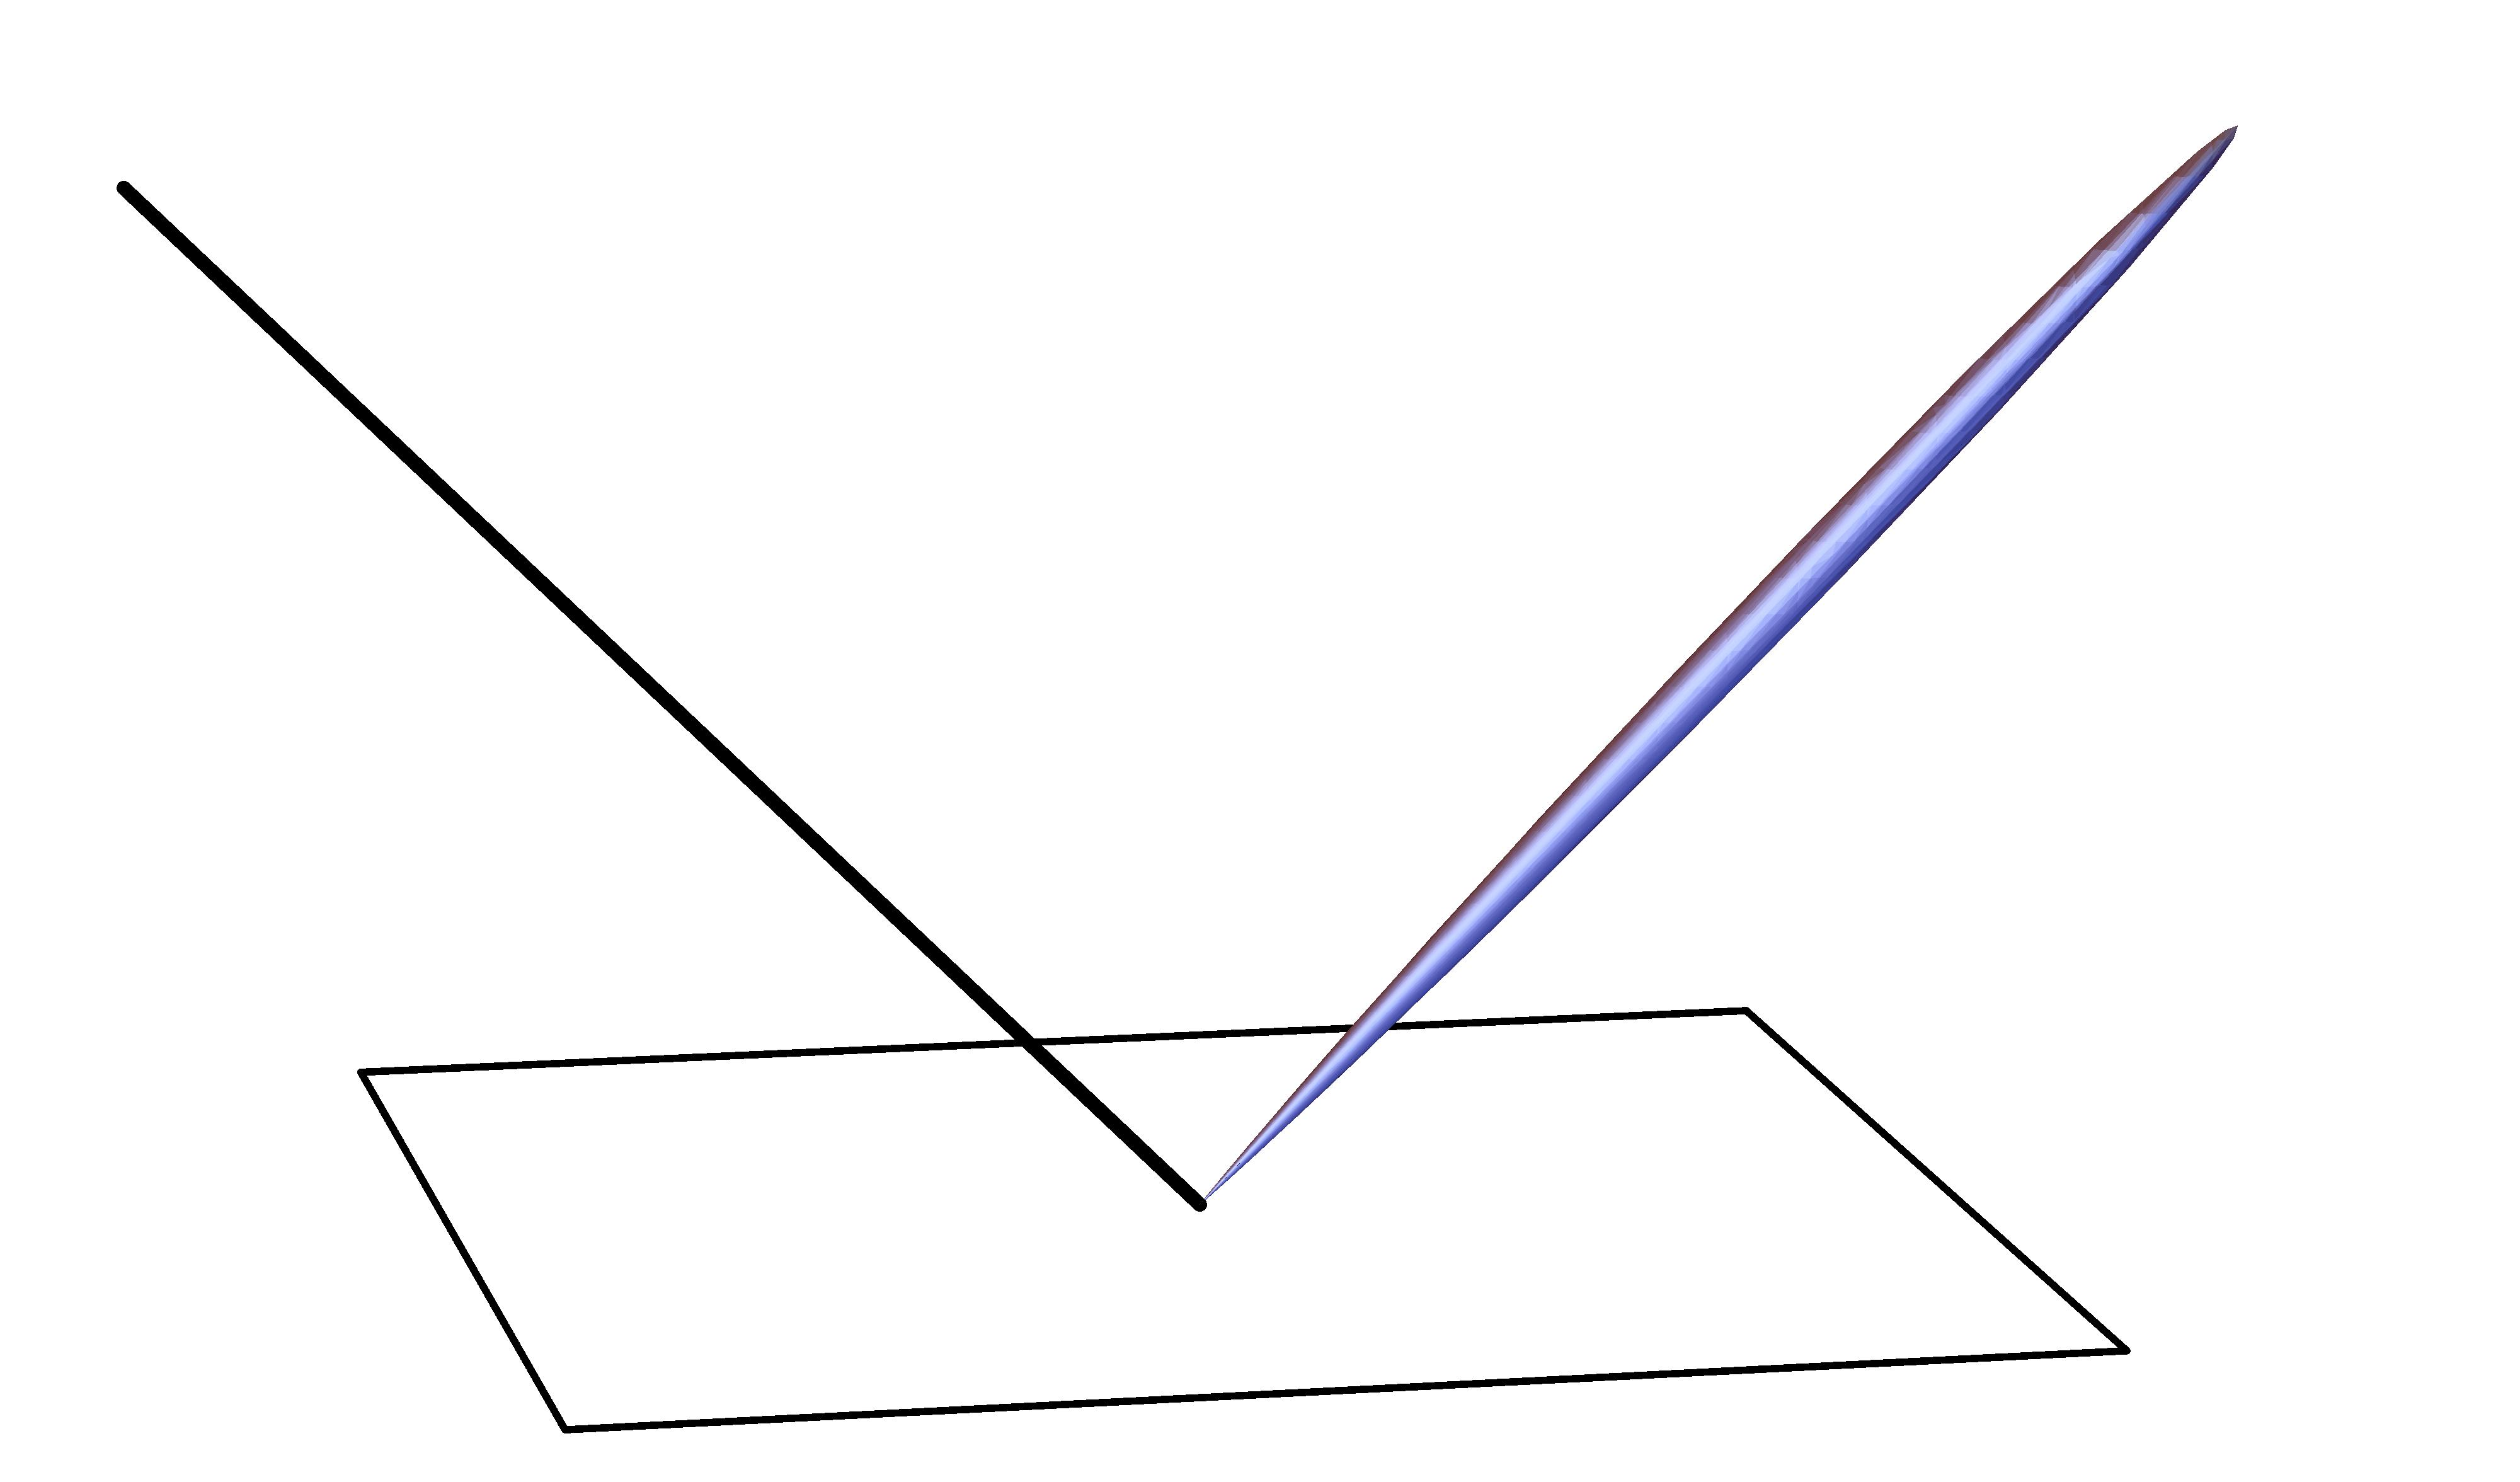
\includegraphics[width=0.5\linewidth]{chap08/brdf-specular-plot.jpg}\label{fig:8.1.3}}
      \subfloat[逆反射BRDF]{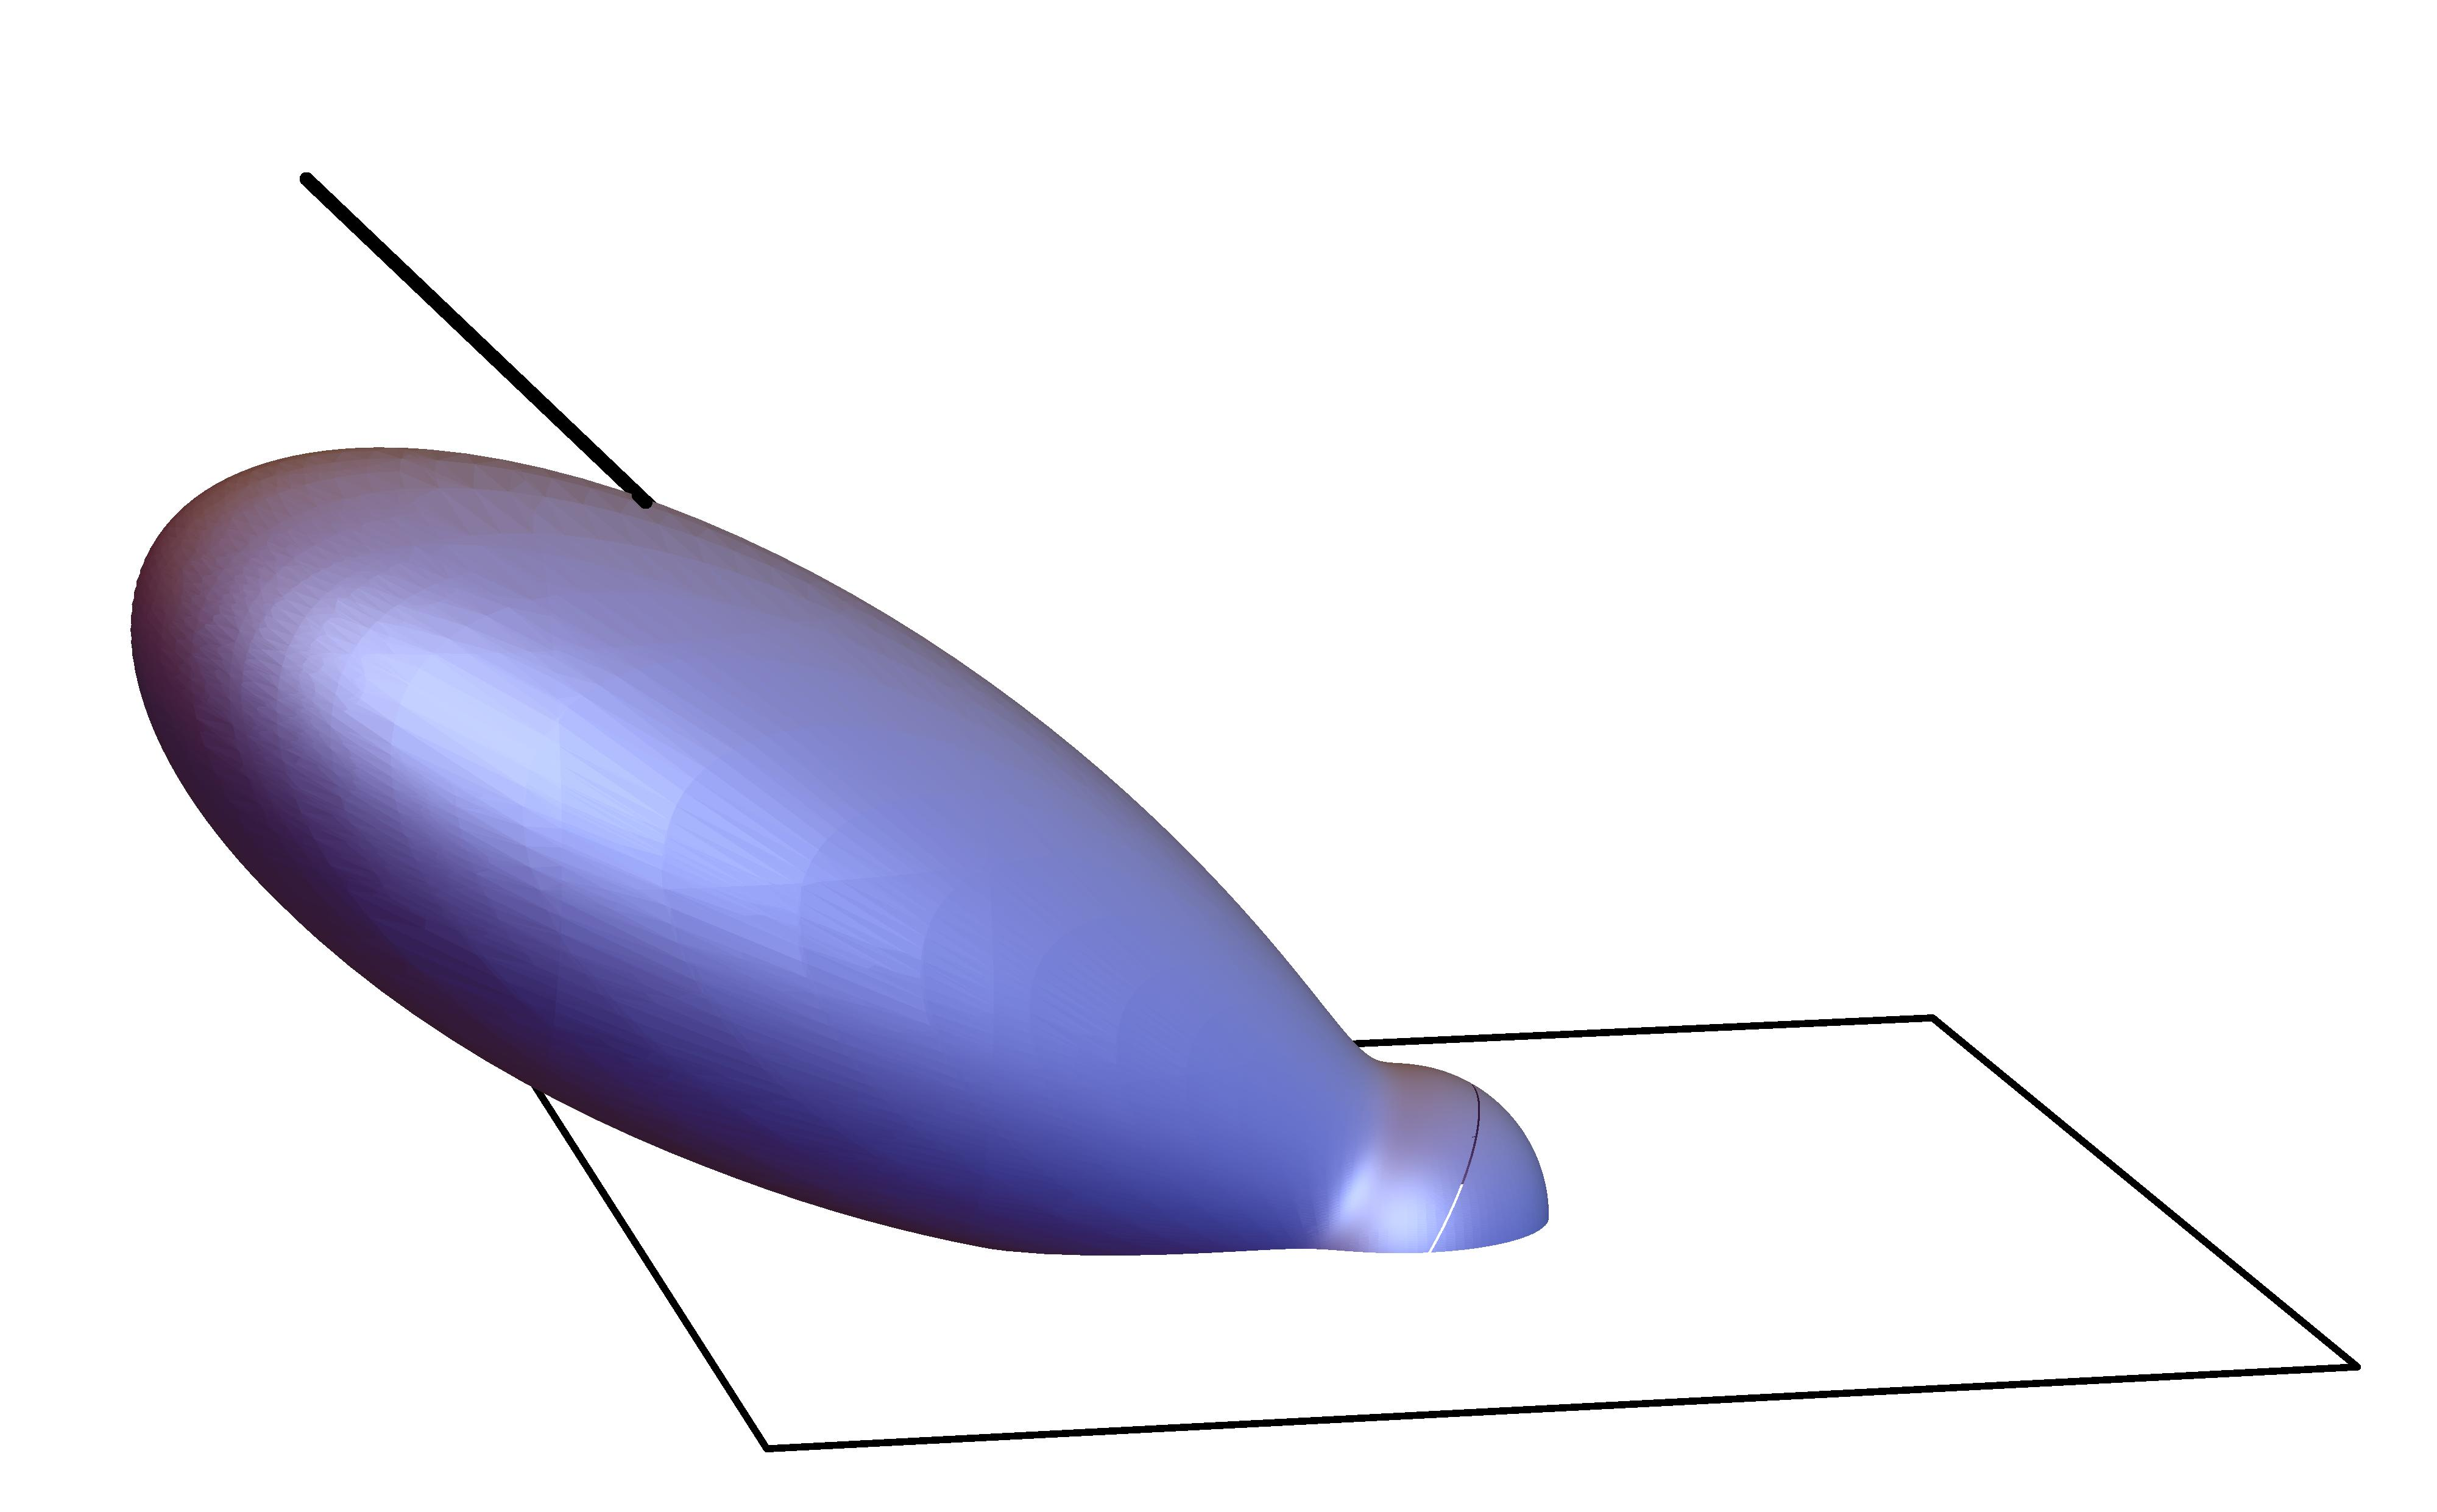
\includegraphics[width=0.5\linewidth]{chap08/brdf-retro-plot.jpg}\label{fig:8.1.4}}
      \caption{来自表面的反射通常可按反射光相对于入射方向(粗线)的分布来划分:
            (1)漫反射、(2)光泽镜面、(3)几乎完美的镜面、(4)逆反射分布。}
      \label{fig:8.1}
\end{figure}

对于特定的某种反射,反射分布函数可能是\keyindex{各向同性}{isotropic}{}
或\keyindex{各向异性}{anisotropic}{}的。大部分物体是各向同性的:
如果你在表面上选一点并绕该处的法线轴旋转它,反射光的分布不变。
相反,当你像这样旋转各向异性材料时,它们反射的光量会不同。
各向异性表面的例子包括拉丝金属、多种布料和压缩光盘。

\subsection{几何设置}\label{sub:几何设置}
pbrt中的反射计算是在反射坐标系中进行的,
被着色点的两个切向量和法向量分别对齐到$x$、$y$和$z$轴(\reffig{8.2})。
所有传入BRDF和BTDF例程及其返回的各方向向量都在该坐标系下定义。
为了理解本章的BRDF和BTDF实现,理解该坐标系很重要。
\begin{figure}[htbp]
      \centering
      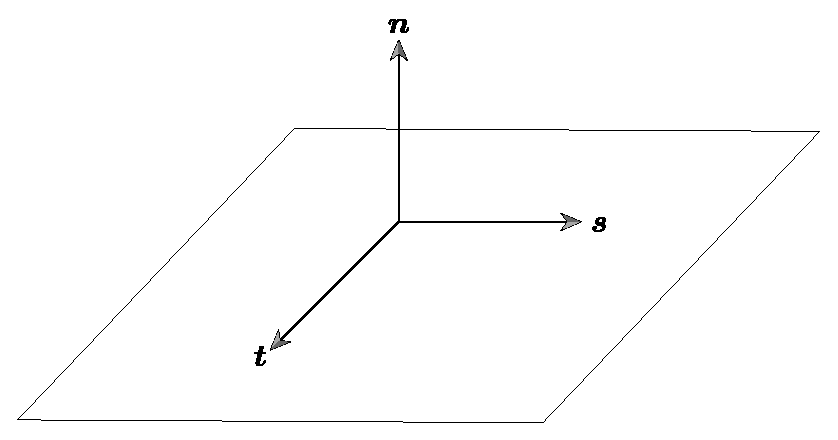
\includegraphics[width=0.7\linewidth]{chap08/BSDFcoordinatesystem.eps}
      \caption{基本BSDF接口设置。着色坐标系由正交基向量$({\bm s},{\bm t},{\bm n})$定义。
            我们将调整这些向量朝向使得它们在该坐标系中沿着$x$、$y$和$z$轴。
            在调用任何BRDF或BTDF方法前,世界空间中的方向向量$\bm \omega$会被
            变换到着色坐标系。}
      \label{fig:8.2}
\end{figure}

着色坐标系也给出了表示球面坐标$(\theta,\varphi)$中方向的坐标系;
角度$\theta$从给定方向测量到$z$轴,$\varphi$是方向投影到$xy$平面后
与$x$轴所成角度。给定该坐标系下的方向向量$\bm\omega$,
很容易计算与法向夹角的余弦等量:
\begin{align*}
      \cos\theta=({\bm n}\cdot{\bm\omega})=((0,0,1)\cdot{\bm\omega})=\omega_z\, .
\end{align*}

我们将提供实用函数来计算这些值和一些有用的变量;
它们的使用有助于阐明BRDF和BTDF的实现。
\begin{lstlisting}
`\initcode{BSDF Inline Functions}{=}\initnext{BSDFInlineFunctions}`
inline `\refvar{Float}{}` `\initvar{CosTheta}{}`(const `\refvar{Vector3f}{}` &w) { return w.z; }
inline `\refvar{Float}{}` `\initvar{Cos2Theta}{}`(const `\refvar{Vector3f}{}` &w) { return w.z * w.z; }
inline `\refvar{Float}{}` `\initvar{AbsCosTheta}{}`(const `\refvar{Vector3f}{}` &w) { return std::abs(w.z); }
\end{lstlisting}

$\sin^2\theta$的值可用三角恒等式$\sin^2\theta+\cos^2\theta=1$算得,
但我们要注意避免取负数的平方根,罕见情况下浮点舍入误差
会让{\ttfamily 1 - \refvar{Cos2Theta}{}(w)}小于零。
\begin{lstlisting}
`\refcode{BSDF Inline Functions}{+=}\lastnext{BSDFInlineFunctions}`
inline `\refvar{Float}{}` `\initvar{Sin2Theta}{}`(const `\refvar{Vector3f}{}` &w) {
    return std::max((`\refvar{Float}{}`)0, (`\refvar{Float}{}`)1 - `\refvar{Cos2Theta}{}`(w));
}
inline `\refvar{Float}{}` `\initvar{SinTheta}{}`(const `\refvar{Vector3f}{}` &w) {
    return std::sqrt(`\refvar{Sin2Theta}{}`(w));
}
\end{lstlisting}

角$\theta$的正切可以由恒等式$\displaystyle\tan\theta=\frac{\sin\theta}{\cos\theta}$计算。
\begin{lstlisting}
`\refcode{BSDF Inline Functions}{+=}\lastnext{BSDFInlineFunctions}`
inline `\refvar{Float}{}` `\initvar{TanTheta}{}`(const `\refvar{Vector3f}{}` &w) {
    return `\refvar{SinTheta}{}`(w) / `\refvar{CosTheta}{}`(w);
}
inline `\refvar{Float}{}` `\initvar{Tan2Theta}{}`(const `\refvar{Vector3f}{}` &w) {
    return `\refvar{Sin2Theta}{}`(w) / `\refvar{Cos2Theta}{}`(w);
}
\end{lstlisting}

我们可以类似地用着色坐标系来简化角$\varphi$的正余弦计算(\reffig{8.3})。
在被着色点的平面内,向量$\bm\omega$的坐标$(x,y)$分别由$r\cos\varphi$和$r\sin\varphi$给出。
半径$r$是$\sin\theta$,所以
\begin{align*}
      \cos\varphi & =\frac{x}{r}=\frac{x}{\sin\theta}\,   \\
      \sin\varphi & =\frac{y}{r}=\frac{y}{\sin\theta}\, .
\end{align*}

\begin{figure}[htbp]
      \centering
      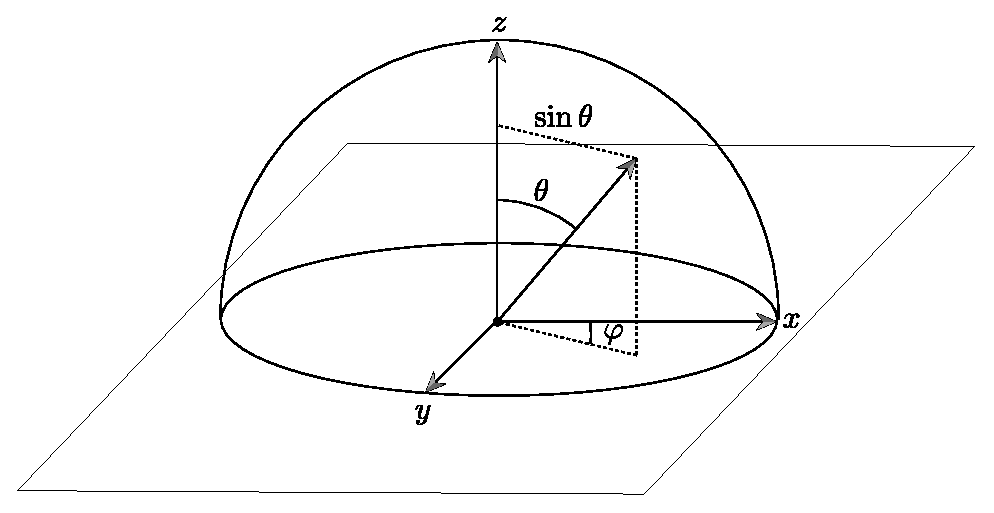
\includegraphics[width=0.7\linewidth]{chap08/BSDFthetaphiangles.eps}
      \caption{$\sin\varphi$和$\cos\varphi$的值可用球面坐标
            方程$x=r\cos\varphi$和$y=r\sin\varphi$算得,其中$r$是虚线的长度,等于$\sin\theta$.}
      \label{fig:8.3}
\end{figure}

\begin{lstlisting}
`\refcode{BSDF Inline Functions}{+=}\lastnext{BSDFInlineFunctions}`
inline `\refvar{Float}{}` `\initvar{CosPhi}{}`(const `\refvar{Vector3f}{}` &w) {
    `\refvar{Float}{}` sinTheta = `\refvar{SinTheta}{}`(w);
    return (sinTheta == 0) ? 1 : `\refvar{Clamp}{}`(w.x / sinTheta, -1, 1);
}
inline `\refvar{Float}{}` `\initvar{SinPhi}{}`(const `\refvar{Vector3f}{}` &w) {
    `\refvar{Float}{}` sinTheta = `\refvar{SinTheta}{}`(w);
    return (sinTheta == 0) ? 0 : `\refvar{Clamp}{}`(w.y / sinTheta, -1, 1);
}
\end{lstlisting}
\begin{lstlisting}
`\refcode{BSDF Inline Functions}{+=}\lastnext{BSDFInlineFunctions}`
inline `\refvar{Float}{}` `\initvar{Cos2Phi}{}`(const `\refvar{Vector3f}{}` &w) {
    return `\refvar{CosPhi}{}`(w) * `\refvar{CosPhi}{}`(w);
}
inline `\refvar{Float}{}` `\initvar{Sin2Phi}{}`(const `\refvar{Vector3f}{}` &w) {
    return `\refvar{SinPhi}{}`(w) * `\refvar{SinPhi}{}`(w);
}
\end{lstlisting}

两个向量在着色坐标系下$\varphi$值间的角$\Delta\varphi$的余弦
可以通过置零两个向量的$z$坐标获得2D向量后再规范化求得。
这两个向量的点积给出了它们夹角的余弦。
为了高效,下面的实现重新排列了项使得只需执行一次平方根运算。
\begin{lstlisting}
`\refcode{BSDF Inline Functions}{+=}\lastnext{BSDFInlineFunctions}`
inline `\refvar{Float}{}` `\initvar{CosDPhi}{}`(const `\refvar{Vector3f}{}` &wa, const `\refvar{Vector3f}{}` &wb) {
    return `\refvar{Clamp}{}`((wa.x * wb.x + wa.y * wb.y) /
                 std::sqrt((wa.x * wa.x + wa.y * wa.y) *
                           (wb.x * wb.x + wb.y * wb.y)), -1, 1);
}
\end{lstlisting}

当阅读本章代码和向pbrt增添BRDF和BTDF时,需要记住一些重要约定和实现细节。
\begin{itemize}
      \item 入射光方向${\bm\omega}_{\mathrm{i}}$和出射查看方向${\bm\omega}_{\mathrm{o}}$都是
            规范化的,且变换到表面的局部坐标系后都是朝外指的。
      \item 按pbrt的约定,曲面法线$\bm n$总是指向物体的“外侧”,这让确定光是进入还是射出透明物体更简单:
            如果入射光方向${\bm\omega}_{\mathrm{i}}$和$\bm n$在同一半球,
            则光在射入;否则光在射出。因此,要记住的一个细节是法线可能相对于
            一个或两个方向向量${\bm\omega}_{\mathrm{i}}$和${\bm\omega}_{\mathrm{o}}$
            在表面的对侧。不像许多其他渲染器那样,pbrt不会翻转法线使其和${\bm\omega}_{\mathrm{o}}$在同侧。
      \item 用于着色的局部坐标系可能并不和来自第\refchap{形状}的例程\refvar{Shape::Intersect}{()}
            返回的坐标系一样;它们在相交和着色间为了达到凹凸贴图等效果可能会被修改。见第\refchap{材质}这类修改的例子。
      \item 最后,BRDF和BTDF的实现不应关心${\bm\omega}_{\mathrm{i}}$和${\bm\omega}_{\mathrm{o}}$是否在同一半球。
            例如,尽管反射BRDF原则上应该检测是否入射方向在表面之上而出射方向在下面并在这种情况下总是不返回反射,
            但这里我们希望反射函数代之以利用其反射模型的合适公式计算和返回反射的光量,
            忽略它们不在同一半球的细节。pbrt中的高层级代码会保证只有反射或透射散射例程会适当求值。
            该约定的价值将在\refsec{BSDF}解释。
\end{itemize}

\section{基本接口}\label{sec:基本接口}
我们将首先定义单个BRDF和BTDF函数的接口。
BRDF和BTDF共享共同的基类\refvar{BxDF}{}。
因为两者都有一样的接口,共享相同的基类减少了重复代码并
允许系统的一些部分和一般的\refvar{BxDF}{}配合而不用区分BRDF和BTDF。
\begin{lstlisting}
`\initcode{BxDF Declarations}{=}\initnext{BxDFDeclarations}`
class `\initvar{BxDF}{}` {
public:
    `\refcode{BxDF Interface}{}`
    `\refcode{BxDF Public Data}{}`
};
\end{lstlisting}

\refsec{BSDF}将要介绍的类\refvar{BSDF}{}持有一系列\refvar{BxDF}{}对象
来一起描述表面上一点的散射。尽管我们把\refvar{BxDF}{}的实现细节隐藏到
反射和透射材质的公共接口后,第\refchap{光传输I:表面反射}到\refchap{光传输III:双向方法}的
一些光传输算法还是需要区分这两个类型。因此,所有\refvar{BxDF}{}都
有成员\refvar{BxDF::type}{}持有来自\refvar{BxDFType}{}的标志。
对于每个\refvar{BxDF}{},该标志应至少有一个置为\refvar[BSDFREFLECTION]{BSDF\_REFLECTION}{}
或\refvar[BSDFTRANSMISSION]{BSDF\_TRANSMISSION}{},且恰有一个漫反射、光泽或镜面标志。
注意没有逆反射标志;这里的分类中逆反射被当作光泽反射。

\begin{lstlisting}
`\initcode{BSDF Declarations}{=}\initnext{BSDFDeclarations}`
enum `\initvar{BxDFType}{}` {
    `\initvar[BSDFREFLECTION]{BSDF\_REFLECTION}{}` = 1 << 0,
    `\initvar[BSDFTRANSMISSION]{BSDF\_TRANSMISSION}{}` = 1 << 1,
    `\initvar[BSDFDIFFUSE]{BSDF\_DIFFUSE}{}` = 1 << 2,
    `\initvar[BSDFGLOSSY]{BSDF\_GLOSSY}{}` = 1 << 3,
    `\initvar[BSDFSPECULAR]{BSDF\_SPECULAR}{}` = 1 << 4,
    `\initvar[BSDFALL]{BSDF\_ALL}{}` = BSDF_DIFFUSE | BSDF_GLOSSY | BSDF_SPECULAR |
                        BSDF_REFLECTION | BSDF_TRANSMISSION,
};
\end{lstlisting}

\begin{lstlisting}
`\initcode{BxDF Interface}{=}\initnext{BxDFInterface}`
`\refvar{BxDF}{}`(`\refvar{BxDFType}{}` type) : `\refvar[BxDF::type]{type}{}`(type) { }
\end{lstlisting}

\begin{lstlisting}
`\initcode{BxDF Public Data}{=}`
const `\refvar{BxDFType}{}` `\initvar[BxDF::type]{type}{}`;
\end{lstlisting}

实用方法\refvar{MatchesFlags}{()}确定\refvar{BxDF}{}是否匹配用户提供的类型标志:
\begin{lstlisting}
`\refcode{BxDF Interface}{+=}\lastnext{BxDFInterface}`
bool `\initvar{MatchesFlags}{}`(`\refvar{BxDFType}{}` t) const {
    return (`\refvar[BxDF::type]{type}{}` & t) == `\refvar[BxDF::type]{type}{}`;
}
\end{lstlisting}

\refvar{BxDF}{}提供的关键方法是\refvar{BxDF::f}{()}。
它为给定的方向对返回分布函数的值。该接口隐式假设了不同波长的光是解耦的——
某一波长的能量不会反射成不同波长。通过作出该假设,反射函数的效应可以直接用\refvar{Spectrum}{}表示。
支持该假设不成立的荧光材料则要求该方法返回一个$n\times n$矩阵以编码光谱样本间的能量转化
(其中$n$是\refvar{Spectrum}{}表示中的样本数量)。
\begin{lstlisting}
`\refcode{BxDF Interface}{+=}\lastnext{BxDFInterface}`
virtual `\refvar{Spectrum}{}` `\initvar[BxDF::f]{f}{}`(const `\refvar{Vector3f}{}` &wo, const `\refvar{Vector3f}{}` &wi) const = 0;
\end{lstlisting}

不是所有\refvar{BxDF}{}都能用方法\refvar[BxDF::f]{f}{()}求值。
例如,像镜子、玻璃或水那样的完美镜面物体只把来自单个入射方向的光朝单个出射方向散射。
这样的\refvar{BxDF}{}最好用$\delta$分布描述,即除了光散射的单个方向外都取零。
pbrt中这些\refvar{BxDF}{}需要特殊处理,所以我们也会提供方法\refvar[BxDF::Samplef]{BxDF::Sample\_f}{()}。
该方法既能用于处理由$\delta$分布描述的散射,
也能从散射光有多个方向的\refvar{BxDF}{}中随机采样方向;
第二种应用将在\refsec{采样反射函数}中讨论蒙特卡罗BSDF采样时解释。

\refvar[BxDF::Samplef]{BxDF::Sample\_f}{()}计算给定出射方向${\bm\omega}_{\mathrm{o}}$的
入射光方向${\bm\omega}_{\mathrm{i}}$并为这对方向返回\refvar{BxDF}{}的值。
对于$\delta$分布,\refvar{BxDF}{}有必要这样选择入射光方向,因为调用者
无法生成合适的方向${\bm\omega}_{\mathrm{i}}$
\footnote{反射函数中的$\delta$分布对于光传输算法有一些额外微妙的影响。
    \refsub{镜面反射与透射}和\refsub{被积函数中的delta分布}详细描述了该问题。}。
$\delta$分布的\refvar{BxDF}{}不需要参数{\ttfamily sample}和{\ttfamily pdf},
所以它们会在后面的\refsec{采样反射函数}解释,到时我们将为非镜面反射函数提供该方法的实现。
\begin{lstlisting}
`\refcode{BxDF Interface}{+=}\lastnext{BxDFInterface}`
virtual `\refvar{Spectrum}{}` `\initvar[BxDF::Samplef]{Sample\_f}{}`(const `\refvar{Vector3f}{}` &wo, `\refvar{Vector3f}{}` *wi,
    const `\refvar{Point2f}{}` &sample, `\refvar{Float}{}` *pdf,
    `\refvar{BxDFType}{}` *sampledType = nullptr) const;
\end{lstlisting}

\subsection{反射}\label{sub:反射}
将4D的BRDF或BTDF的表现聚合起来定义为一对方向上的函数,
并将其简化为单个方向上的2D函数甚至是描述其整体散射表现的常数值很有用。

\keyindex{半球定向反射率}{hemispherical-directional reflectance}{}是
一个2D函数,它给出了半球上常量照明于给定方向上的反射率,
或者等价地,因来自给定方向的光而在半球上的总反射率
\footnote{这两个量相等的事实源自反射函数的互易性。BTDF通常不互易;见\refsub{非对称散射}。}。
它定义为
\begin{align}
    \label{eq:8.1}
    \rho_{\mathrm{hd}}({\bm\omega}_{\mathrm{o}})=\int_{H^2({\bm n})}{f_{\mathrm{r}}({\bm p},{\bm \omega}_\mathrm{o},{\bm \omega}_\mathrm{i})|\cos{\theta_{\mathrm{i}}}|\mathrm{d}{\bm \omega}_\mathrm{i}}\, .
\end{align}

方法\refvar{BxDF::rho}{()}计算反射函数$\rho_{\mathrm{hd}}$.
一些\refvar{BxDF}{}能解析地计算该值,然而大部分用蒙特卡罗积分来计算其近似值。
对于那些\refvar{BxDF}{},参数{\ttfamily nSamples}和{\ttfamily samples}供
蒙特卡罗算法的实现使用;它们将在\refsub{应用:估计反射率}解释。
\begin{lstlisting}
`\refcode{BxDF Interface}{+=}\lastnext{BxDFInterface}`
virtual `\refvar{Spectrum}{}` `\initvar[BxDF::rho]{rho}{}`(const `\refvar{Vector3f}{}` &wo, int nSamples,
                     const `\refvar{Point2f}{}` *samples) const;
\end{lstlisting}

表面的\keyindex{半球半球反射率}{hemispherical-hemispherical reflectance}{}记为$\rho_{\mathrm{hh}}$,
该光谱值给出了当各方向入射光相同时表面反射的入射光比例。它是
\begin{align*}
    \rho_{\mathrm{hh}}=\frac{1}{\pi}\int_{H^2({\bm n})}\int_{H^2({\bm n})}f_{\mathrm{r}}({\bm p},{\bm \omega}_\mathrm{o},{\bm \omega}_\mathrm{i})|\cos{\theta_{\mathrm{o}}}\cos{\theta_{\mathrm{i}}}|\mathrm{d}{\bm \omega}_\mathrm{o}\mathrm{d}{\bm \omega}_\mathrm{i}\, .
\end{align*}

如果不提供方向${\bm\omega}_\mathrm{o}$,则方法\refvar[BxDF::rho2]{BxDF::rho}{()}计算$\rho_{\mathrm{hh}}$.
剩下的参数又是在需要时用于计算$\rho_{\mathrm{hh}}$值的蒙特卡罗估计。
\begin{lstlisting}
`\refcode{BxDF Interface}{+=}\lastcode{BxDFInterface}`
virtual `\refvar{Spectrum}{}` `\initvar[BxDF::rho2]{rho}{}`(int nSamples, const `\refvar{Point2f}{}` *samples1,
                     const `\refvar{Point2f}{}` *samples2) const;
\end{lstlisting}

\subsection{BxDF缩放适配器}\label{sub:BxDF缩放适配器}
取一个给定的\refvar{BxDF}{}并用一个\refvar{Spectrum}{}值
缩放它的作用也很有用。\refvar{ScaledBxDF}{}
封装器持有一个\refvar{BxDF}{*}和\refvar{Spectrum}{}并实现其功能。
该类由\refvar{MixMaterial}{}(定义于\refsub{混合材料})使用,
它基于另两种材料的加权和创建\refvar{BSDF}{}。
\begin{lstlisting}
`\refcode{BxDF Declarations}{+=}\lastnext{BxDFDeclarations}`
class `\initvar{ScaledBxDF}{}` : public `\refvar{BxDF}{}` {
public:
    `\refcode{ScaledBxDF Public Methods}{}`
private:
    `\refvar{BxDF}{}` *`\initvar[ScaledBxDF::bxdf]{bxdf}{}`;
    `\refvar{Spectrum}{}` `\initvar[ScaledBxDF::scale]{scale}{}`;
};
\end{lstlisting}
\begin{lstlisting}
`\initcode{ScaledBxDF Public Methods}{=}`
`\refvar{ScaledBxDF}{}`(`\refvar{BxDF}{}` *bxdf, const `\refvar{Spectrum}{}` &scale)
    : `\refvar{BxDF}{}`(`\refvar{BxDFType}{}`(bxdf->`\refvar[BxDF::type]{type}{}`)), `\refvar[ScaledBxDF::bxdf]{bxdf}{}`(bxdf), `\refvar[ScaledBxDF::scale]{scale}{}`(scale) {
}
\end{lstlisting}

\refvar{ScaledBxDF}{}的方法实现很简单;我们这里只介绍\refvar[ScaledBxDF::f]{f}{()}。
\begin{lstlisting}
`\initcode{BxDF Method Definitions}{=}\initnext{BxDFMethodDefinitions}`
`\refvar{Spectrum}{}` `\refvar{ScaledBxDF}{}`::`\initvar[ScaledBxDF::f]{f}{}`(const `\refvar{Vector3f}{}` &wo, const `\refvar{Vector3f}{}` &wi) const {
    return `\refvar[ScaledBxDF::scale]{scale}{}` * `\refvar[ScaledBxDF::bxdf]{bxdf}{}`->`\refvar[BxDF::f]{f}{}`(wo, wi);
}
\end{lstlisting}

\section{镜面反射与透射}\label{sec:镜面反射与透射}

绝对光滑表面上光的特性较容易用物理和几何光学模型分析刻画。
这些表面展现出入射光的完美镜像反射和透射;
对于给定的方向${\bm\omega}_{\mathrm{i}}$,
所有光都散射到单个出射方向${\bm\omega}_{\mathrm{o}}$.
对于镜面反射,该出射方向和法线所成角与入射方向相同:
\begin{align*}
    \theta_{\mathrm{i}}=\theta_{\mathrm{o}}\, ,
\end{align*}
且其中$\varphi_{\mathrm{o}}=\varphi_{\mathrm{i}}+\pi$.
对于透射,我们也有$\varphi_{\mathrm{o}}=\varphi_{\mathrm{i}}+\pi$,
且出射方向$\theta_{\mathrm{t}}$由斯涅尔定律给出,
它将折射方向与曲面法线$\bm n$的夹角$\theta_{\mathrm{t}}$与
入射光线与曲面法线$\bm n$的夹角$\theta_{\mathrm{i}}$联系起来
(本章末的习题之一是用光学的费马原理推导斯涅尔定律)。
斯涅尔定律基于入射光线所在介质的\keyindex{折射率}{index of refraction}{}和
要进入的介质的折射率。折射率描述了光在特定介质中相比在真空中传播要慢多少。
我们用希腊字母$\eta$表示折射率,读作“eta”。斯涅尔定律是
\begin{align}
    \label{eq:8.2}
    \eta_{\mathrm{i}}\sin\theta_{\mathrm{i}}=\eta_{\mathrm{t}}\sin\theta_{\mathrm{t}}\, .
\end{align}

通常,折射率随波长变化。因此,在两种不同介质界面上入射光通常散射到多个方向,
该效应称为\keyindex{色散}{dispersion}{}。
当入射白光被棱镜分出光谱成分时可以观察到该效应。
图形学中的通行做法是忽略该波长依赖性,
因为该效应通常对视觉准确性并不关键且忽略它能极大简化光传输计算。
可选地,可以在有色散物体的环境中追踪多束光路(例如一系列离散波长)。
第\refchap{光传输I:表面反射}末的“扩展阅读”一节有关于该话题的更多信息指引。
\begin{figure}[htbp]
    \centering
    \subfloat[镜面反射]{\includegraphics[width=0.75\linewidth]{chap08/dragon-specular-reflect.png}\label{fig:8.4.1}}\\
    \subfloat[镜面透射]{\includegraphics[width=0.75\linewidth]{chap08/dragon-specular-transmit.png}\label{fig:8.4.2}}
    \caption{用(1)完美镜面反射和(2)完美镜面折射渲染的龙模型。图像(2)排除了
        内外反射的影响;导致的能量损失产生了显眼的暗区(感谢Christian Schüller提供模型)。}
    \label{fig:8.4}
\end{figure}

\reffig{8.4}展示了完美镜面反射和透射的效果。

\subsection{菲涅尔反射率}\label{sub:菲涅尔反射率}
除了反射和透射方向,还有必要计算反射或透射的入射光占比。
为了物理上准确反射或折射,该项依赖于方向,而不能用每个表面的缩放常数表征。
\keyindex{菲涅耳方程}{Fresnel equations}{}
\sidenote{译者注:得名于法国物理学家奥古斯丁·菲涅耳(Augustin-Jean Fresnel)。}描述了
表面上反射光的量;它们是麦克斯韦方程在光滑表面上的解。

给定折射率和入射光与曲面法线所成角度,菲涅耳方程
指定了材料对两种不同偏振状态的入射照明相应的反射率。
因为偏振的视觉效果在大多数环境下是受限的,
所以在pbrt中我们将作出光是无偏振的常用假设;
即光波是随机朝向的。有了该简化假设,菲涅尔反射率就是
平行和垂直偏振项的均方。

此刻有必要指出几个重要材料类别的差异:
\begin{enumerate}
    \item 第一类是\keyindex{介电质}{dielectric}{},
          是不会导电的材料。它们有实数值的折射率(通常在范围1-3内)且
          透射\footnote{注意介电质可能充满能吸收大部分或所有透射光的粒子(例如石油)。
              像水那样的介电质也能通过添加离子使之导电而变成电解质溶液。
              这两方面都和材料本身划分为介电质或导体无关。}一部分入射照明。
          介电质的例子有玻璃、矿油、水和空气。
    \item 第二类组成是\keyindex{导体}{conductor}{}例如金属。
          价电子可以自由地在原子晶格中移动,允许电流从一个地方流到另一处。
          当导体受到电磁辐射例如可见光时,这一基本的原子属性就会转化为完全不同的特性:
          该材料是不透明的并反射回大部分照明。一部分光也透射进导体内部并被迅速吸收:
          总吸收通常发生在材料表面0.1$\mu\mathrm{m}$内,因此只有极薄的金属膜才能透射足够的光量。
          我们在pbrt中忽略该效应而只建模导体的反射部分。与介电质相反,
          导体有复数值的折射率$\bar{\eta}=\eta+\mathrm{i}k$.
    \item \keyindex{半导体}{semiconductor}{}例如硅或锗是本书中我们不予考虑的第三类。
\end{enumerate}

导体和介电质都由同一组菲涅尔方程表征。
尽管如此,我们更喜欢为介电质创建特殊的求值函数,
这样当折射率保证为实数值时,这些方程会取特别简单的形式。

\begin{table}[htbp]
    \centering
    \begin{tabular}{ll}
        \toprule
        \textbf{介质}  & \textbf{折射率}$\eta$ \\
        \midrule
        真空           & 1.0                   \\
        海平面上的空气 & 1.00029               \\
        冰             & 1.31                  \\
        水(20℃)      & 1.333                 \\
        熔融石英       & 1.46                  \\
        玻璃           & 1.5-1.6               \\
        蓝宝石         & 1.77                  \\
        钻石           & 2.42                  \\
        \bottomrule
    \end{tabular}
    \caption{各种物体的折射率,给出了光在真空中的速度与
        光在介质中的速度的比值。它们通常是与波长相关的量;
        这些值是在可见波长上的均值。}
    \label{tab:8.1}
\end{table}

为了计算两种介电质界面处的菲涅尔反射率,我们
需要知道这两种介质的折射率。\reftab{8.1}有许多介电质的折射率。
介电质的菲涅尔反射率公式是
\begin{align*}
    r_{\parallel} & =\frac{\eta_{\mathrm{t}}\cos\theta_{\mathrm{i}}-\eta_{\mathrm{i}}\cos\theta_{\mathrm{t}}}{\eta_{\mathrm{t}}\cos\theta_{\mathrm{i}}+\eta_{\mathrm{i}}\cos\theta_{\mathrm{t}}}\, , \\
    r_{\perp}     & =\frac{\eta_{\mathrm{i}}\cos\theta_{\mathrm{i}}-\eta_{\mathrm{t}}\cos\theta_{\mathrm{t}}}{\eta_{\mathrm{i}}\cos\theta_{\mathrm{i}}+\eta_{\mathrm{t}}\cos\theta_{\mathrm{t}}}\, ,
\end{align*}
其中$r_{\parallel}$是平行偏振光的菲涅尔反射率,
$r_{\perp}$是垂直偏振光的反射率,$eta_{\mathrm{i}}$和$\eta_{\mathrm{t}}$是
入射和透射介质的折射率,$\bm\omega_{\mathrm{i}}$和$\bm\omega_{\mathrm{t}}$是
入射和透射方向。$\bm\omega_{\mathrm{t}}$由斯涅尔定律算出(见\refsub{镜面透射})。

余弦项应该大于或等于零;出于计算这些值的目的,
当计算$\cos\theta_{\mathrm{i}}$和$\cos\theta_{\mathrm{t}}$时,
几何法线应该分别翻转到和$\bm\omega_{\mathrm{i}}$或$\bm\omega_{\mathrm{t}}$同侧。

对于非偏振光,菲涅尔反射率是
\begin{align*}
    F_{\mathrm{r}}=\frac{1}{2}(r_{\parallel}^2+r_{\perp}^2)\, .
\end{align*}

因为能量守恒,介电质传输的能量为$1-F_{\mathrm{r}}$.

函数\refvar{FrDielectric}{()}为介电质材料和非偏振光计算菲涅尔反射率公式。
量$\cos\theta_{\mathrm{i}}$作为参数{\ttfamily cosThetaI}传入。
\begin{lstlisting}
`\initcode{BxDF Utility Functions}{=}`
`\refvar{Float}{}` `\initvar{FrDielectric}{}`(`\refvar{Float}{}` cosThetaI, `\refvar{Float}{}` etaI, `\refvar{Float}{}` etaT) {
    cosThetaI = `\refvar{Clamp}{}`(cosThetaI, -1, 1);
    `\refcode{Potentially swap indices of refraction}{}`
    `\refcode{Compute cosThetaT using Snell's law}{}`
    `\refvar{Float}{}` Rparl = ((etaT * cosThetaI) - (etaI * cosThetaT)) /
                  ((etaT * cosThetaI) + (etaI * cosThetaT));
    `\refvar{Float}{}` Rperp = ((etaI * cosThetaI) - (etaT * cosThetaT)) /
                  ((etaI * cosThetaI) + (etaT * cosThetaT));
    return (Rparl * Rparl + Rperp * Rperp) / 2;
}
\end{lstlisting}

为了求得折射角的余弦{\ttfamily cosThetaT},
首先需要确定入射方向是在介质的外面还是里面,这样才能恰当解释两个折射率。

入射角余弦的符号表明了入射光在介质的哪一侧(\reffig{8.5})。
如果余弦在0到1间,则光线在外侧,如果在-1到0间,则光线在内侧。
调整参数{\ttfamily etaI}和{\ttfamily etaT}使得{\ttfamily etaI}
是入射介质的折射率,这样保证了{\ttfamily cosThetaI}非负。

\begin{figure}[htbp]
    \centering
    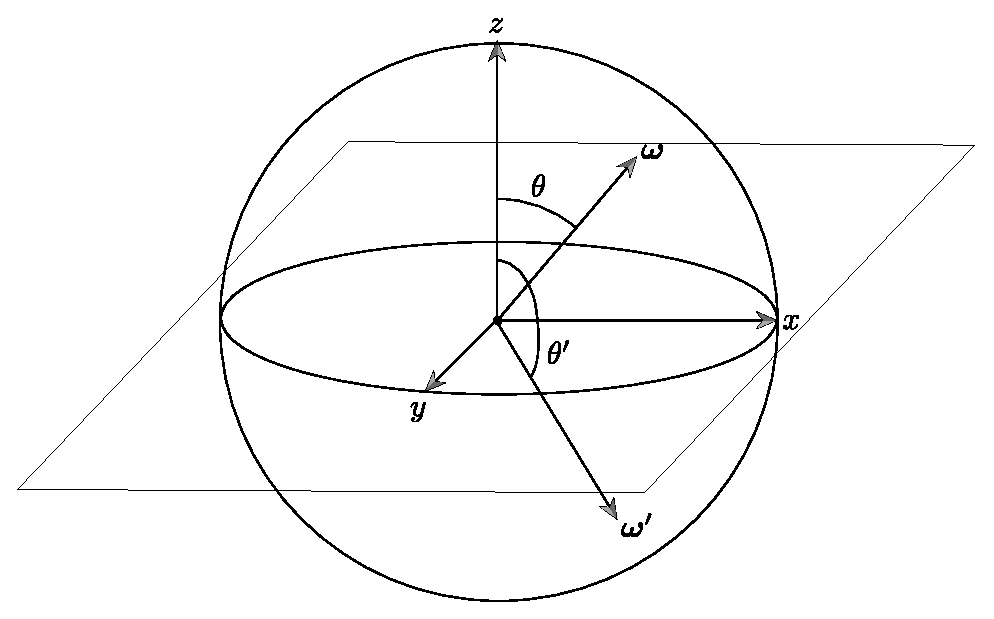
\includegraphics[width=0.7\linewidth]{chap08/BSDFanglegivesinout.eps}
    \caption{方向$\bm\omega$和几何曲面法线间夹角$\theta$的余弦
        表明方向是指向表面外侧(和法线在同一半球)还是表面内侧。
        在标准反射坐标系中,该测试只要求检查方向向量的$z$分量。
        这里,$\bm\omega$在上半球,取正值余弦,而${\bm\omega}'$在下半球。}
    \label{fig:8.5}
\end{figure}

\begin{lstlisting}
`\initcode{Potentially swap indices of refraction}{=}`
bool entering = cosThetaI > 0.f;
if (!entering) {
    std::swap(etaI, etaT);
    cosThetaI = std::abs(cosThetaI);
}
\end{lstlisting}

一旦确定折射率,我们就能用斯涅尔定律(\refeq{8.2})计算
透射方向和曲面法线夹角的正弦$\sin\theta_{\mathrm{t}}$.
最后,用恒等式$\sin^2\theta+\cos^2\theta=1$求得该角的余弦。
\begin{lstlisting}
`\initcode{Compute cosThetaT using Snell's law}{=}`
`\refvar{Float}{}` sinThetaI = std::sqrt(std::max((`\refvar{Float}{}`)0,
                                     1 - cosThetaI * cosThetaI));
`\refvar{Float}{}` sinThetaT = etaI / etaT * sinThetaI;
`\refcode{Handle total internal reflection}{}`
`\refvar{Float}{}` cosThetaT = std::sqrt(std::max((`\refvar{Float}{}`)0,
                                     1 - sinThetaT * sinThetaT));
\end{lstlisting}

当从一种介质传播到另一种折射率更低的介质时,入射角接近掠角的光不能进入另一介质。
发生该现象的最大角称为\keyindex{临界角}{critical angle}{};
当$\theta_{\mathrm{i}}$大于临界角时,发生\keyindex{全内反射}{total internal reflection}{reflection反射},
所有光都被反射。这里通过$\sin\theta_{\mathrm{t}}$大于1检测到该情况;
此时不需要菲涅尔方程。
\begin{lstlisting}
`\initcode{Handle total internal reflection}{=}`
if (sinThetaT >= 1)
    return 1;
\end{lstlisting}

我们现在聚焦一般情况下的复数折射率$\bar{\eta}=\eta+\mathrm{i}k$,
其中一些入射光被材料部分吸收并变为热量。
除了实部,一般菲涅尔公式现在也依赖于虚部$k$,
称为\keyindex{吸收系数}{absorption coefficient}{}。

\reffig{8.6}展示了金的折射率和吸收系数图示。两者都是与波长相关的量。
pbrt发行版中目录{\ttfamily scenes/spds/metals}下有各种金属的$\eta$与$k$与波长相关的数据。
下章的\reffig{9.4}展示了用金属材料渲染的模型。
\begin{figure}[htbp]
    \centering
    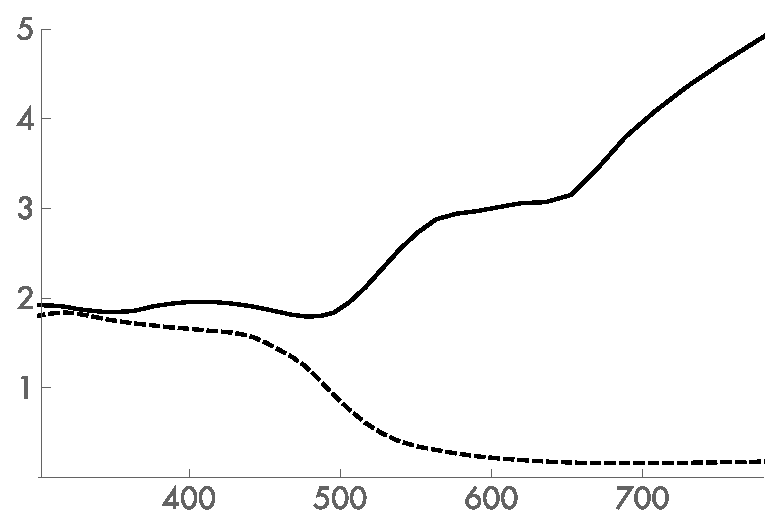
\includegraphics[width=0.7\linewidth]{chap08/au-k-eta.eps}
    \caption{金的吸收系数和折射率。该图展示了金的吸收系数$k$(实线)
        和折射率$\eta$(虚线)随光谱变化的值,横轴是波长,单位纳米。}
    \label{fig:8.6}
\end{figure}

导体和介电质界面处的菲涅尔反射率是
\begin{align}
    \label{eq:8.3}
    r_{\perp}     & =\frac{a^2+b^2-2a\cos\theta+\cos^2\theta}{a^2+b^2+2a\cos\theta+\cos^2\theta}\, ,\nonumber                                                     \\
    r_{\parallel} & =r_{\perp}\frac{(a^2+b^2)\cos^2\theta-2a\cos\theta\sin^2\theta+\sin^4\theta}{(a^2+b^2)\cos^2\theta+2a\cos\theta\sin^2\theta+\sin^4\theta}\, ,
\end{align}
其中
\begin{align*}
    a^2+b^2=\sqrt{(\eta^2-k^2-\sin^2\theta)^2+4\eta^2k^2}\, ,
\end{align*}
且$\displaystyle\eta+\mathrm{i}k=\frac{\bar{\eta_\mathrm{t}}}{\bar{\eta_\mathrm{i}}}$是
用复数除法算出的相对折射率。然而,通常$\bar{\eta_\mathrm{i}}$是介电质的
所以可以替代使用普通的实数除法。

该计算由函数\refvar{FrConductor}{()}实现
\footnote{注意这稍微用词不当,因为函数在技术上包含了介电质$k=0$的情况。
    也就是说,我们选这个名称是为了表明该函数应只用于处理导体,
    因为它比求\refvar{FrDielectric}{()}的开销更大。};
该实现直接对应\refeq{8.3}所以这里不介绍了。
\begin{lstlisting}
`\initcode{Reflection Declarations}{=}`
`\refvar{Spectrum}{}` `\initvar{FrConductor}{}`(`\refvar{Float}{}` cosThetaI, const `\refvar{Spectrum}{}` &etaI,
    const `\refvar{Spectrum}{}` &etaT, const `\refvar{Spectrum}{}` &k);
\end{lstlisting}

为了方便,我们定义抽象类\refvar{Fresnel}{}以提供接口计算菲涅尔反射系数。
用该接口的实现帮助简化后续可能需要支持两种形式的BRDF实现。
\begin{lstlisting}
`\refcode{BxDF Declarations}{+=}\lastnext{BxDFDeclarations}`
class `\initvar{Fresnel}{}` {
public:
    `\refcode{Fresnel Interface}{}`
};
\end{lstlisting}

\refvar{Fresnel}{}接口提供的唯一函数是\refvar{Fresnel::Evaluate}{()}。
给定入射方向和曲面法线夹角的余弦,它返回表面反射的光量。
\begin{lstlisting}
`\initcode{Fresnel Interface}{=}`
virtual `\refvar{Spectrum}{}` `\initvar[Fresnel::Evaluate]{Evaluate}{}`(`\refvar{Float}{}` cosI) const = 0;
\end{lstlisting}

\subsubsection*{菲涅尔导体}
\refvar{FresnelConductor}{}为导体实现该接口。
\begin{lstlisting}
`\refcode{BxDF Declarations}{+=}\lastnext{BxDFDeclarations}`
class `\initvar{FresnelConductor}{}` : public `\refvar{Fresnel}{}` {
public:
    `\refcode{FresnelConductor Public Methods}{}`
private:
    `\refvar{Spectrum}{}` `\initvar[FresnelConductor::etaI]{etaI}{}`, `\initvar[FresnelConductor::etaT]{etaT}{}`, `\initvar[FresnelConductor::k]{k}{}`;
};
\end{lstlisting}

其构造函数存有给定的折射率$\eta$和吸收系数$k$.
\begin{lstlisting}
`\initcode{FresnelConductor Public Methods}{=}`
`\refvar{FresnelConductor}{}`(const `\refvar{Spectrum}{}` &etaI, const `\refvar{Spectrum}{}` &etaT,
    const `\refvar{Spectrum}{}` &k) : `\refvar[FresnelConductor::etaI]{etaI}{}`(etaI), `\refvar[FresnelConductor::etaT]{etaT}{}`(), `\refvar[FresnelConductor::k]{k}{}`(k) { }
\end{lstlisting}

\refvar{FresnelConductor}{}的求值例程也很简单;它只需调用之前定义的函数
\refvar{FrConductor}{()}。注意在调用\refvar{FrConductor}{()}
前{\ttfamily cosThetaI}要取绝对值,因为\refvar{FrConductor}{()}
要求该余弦是在法线和${\bm\omega}_{\mathrm{i}}$在表面的同一侧时测出的,
或者等价地,应该用$\cos\theta_{\mathrm{i}}$的绝对值。
\begin{lstlisting}
`\refcode{BxDF Method Definitions}{+=}\lastnext{BxDFMethodDefinitions}`
`\refvar{Spectrum}{}` `\refvar{FresnelConductor}{}`::`\initvar[FresnelConductor::Evaluate]{Evaluate}{}`(`\refvar{Float}{}` cosThetaI) const {
    return `\refvar{FrConductor}{}`(std::abs(cosThetaI), `\refvar[FresnelConductor::etaI]{etaI}{}`, `\refvar[FresnelConductor::etaT]{etaT}{}`, `\refvar[FresnelConductor::k]{k}{}`);
}
\end{lstlisting}

\subsubsection*{菲涅尔介电质}
\refvar{FresnelDielectric}{}类似地为介电质材料实现了\refvar{Fresnel}{}接口。
\begin{lstlisting}
`\refcode{BxDF Declarations}{+=}\lastnext{BxDFDeclarations}`
class `\initvar{FresnelDielectric}{}` : public `\refvar{Fresnel}{}` {
public:
    `\refcode{FresnelDielectric Public Methods}{}`
private:
    `\refvar{Float}{}` `\initvar[FresnelDielectric::etaI]{etaI}{}`, `\initvar[FresnelDielectric::etaT]{etaT}{}`;
};
\end{lstlisting}

其构造函数存有表面内外侧的折射率。
\begin{lstlisting}
`\initcode{FresnelDielectric Public Methods}{=}`
`\refvar{FresnelDielectric}{}`(`\refvar{Float}{}` etaI, `\refvar{Float}{}` etaT) : `\refvar[FresnelDielectric::etaI]{etaI}{}`(etaI), `\refvar[FresnelDielectric::etaT]{etaT}{}`(etaT) { }
\end{lstlisting}

\refvar{FresnelDielectric}{}的求值例程类似地调用\refvar{FrDielectric}{()}。
\begin{lstlisting}
`\refcode{BxDF Method Definitions}{+=}\lastnext{BxDFMethodDefinitions}`
`\refvar{Spectrum}{}` `\refvar{FresnelDielectric}{}`::`\initvar[FresnelDielectric::Evaluate]{Evaluate}{}`(`\refvar{Float}{}` cosThetaI) const {
    return `\refvar{FrDielectric}{}`(cosThetaI, `\refvar[FresnelDielectric::etaI]{etaI}{}`, `\refvar[FresnelDielectric::etaT]{etaT}{}`);
}
\end{lstlisting}

\subsubsection*{特殊菲涅尔接口}
\refvar{Fresnel}{}接口的实现\refvar{FresnelNoOp}{}对所有入射方向返回100\%反射率。
尽管这在物理上不可实现,但这是可用的方便能力。
\begin{lstlisting}
`\refcode{BxDF Declarations}{+=}\lastnext{BxDFDeclarations}`
class `\initvar{FresnelNoOp}{}` : public `\refvar{Fresnel}{}` {
public:
    `\refvar{Spectrum}{}` `\initvar[FresnelNoOp::Evaluate]{Evaluate}{}`(`\refvar{Float}{}`) const { return `\refvar{Spectrum}{}`(1.); }
};
\end{lstlisting}

\subsection{镜面反射}\label{sub:镜面反射}
我们现在可以实现类\refvar{SpecularReflection}{},
它用菲涅尔接口计算反射光的占比,描述了物理可实现的镜面反射。
首先,我们将推导描述镜面反射的BRDF。
既然菲涅尔方程给出了反射光的比例$F_{\mathrm{r}}({\bm\omega})$,
那么我们需要这样的BRDF
\begin{align*}
    L_{\mathrm{o}}({\bm\omega}_{\mathrm{o}})=\int{f_{\mathrm{r}}({\bm\omega}_{\mathrm{o}},{\bm\omega}_{\mathrm{i}})L_{\mathrm{i}}({\bm\omega}_{\mathrm{i}})|\cos\theta_{\mathrm{i}}|\mathrm{d}{\bm\omega}_{\mathrm{i}}}=F_{\mathrm{r}}({\bm\omega}_{\mathrm{r}})L_{\mathrm{i}}({\bm\omega}_{\mathrm{r}})\, ,
\end{align*}
其中${\bm\omega}_{\mathrm{r}}=R({\bm\omega}_{\mathrm{o}},{\bm n})$是由${\bm\omega}_{\mathrm{o}}$关于
曲面法线$\bm n$反射的镜面反射向量(回想对于镜面反射有$\theta_{\mathrm{r}}=\theta_{\mathrm{o}}$,
因此$F_{\mathrm{r}}({\bm\omega}_{\mathrm{o}})=F_{\mathrm{r}}({\bm\omega}_{\mathrm{r}})$)。

此类BRDF可用狄拉克$\delta$分布构造。
回顾\refsec{采样理论}中$\delta$分布有个好用的性质
\begin{align}\label{eq:8.4}
    \int{f(x)\delta(x-x_0)\mathrm{d}x}=f(x_0)\, .
\end{align}
然而相比于标准函数,$\delta$分布需要特殊处理。
特别地,对有$\delta$分布的积分求数值积分必须显式考虑$\delta$分布。
考虑\refeq{8.4}中的积分:如果我们尝试用梯形法则或
其他一些数值积分技术计算它,则按$\delta$分布的定义,
在任意取值点$x_i$处$\delta(x_i)$为非零值的概率都为零。
确切地说,我们必须允许$\delta$分布自己确定取值点。
我们将在来自特殊\refvar{BxDF}{}的光传输积分以及
第\refchap{光源}的一些光源中遇到$\delta$分布。

直觉上,我们想让镜面反射BRDF在完美反射方向以外任何地方都取零,
这暗示了要用$\delta$分布。首先可能想到的是用$\delta$函数
把入射方向限制到镜面反射方向${\bm\omega}_{\mathrm{r}}$.
这样得到BRDF
\begin{align*}
    f_{\mathrm{r}}({\bm\omega}_{\mathrm{o}},{\bm\omega}_{\mathrm{i}})=\delta_{\mathrm{r}}({\bm\omega}_{\mathrm{i}}-{\bm\omega}_{\mathrm{r}})F_{\mathrm{r}}({\bm\omega}_{\mathrm{i}})\, .
\end{align*}

尽管这看起来很诱人,但把它代入散射方程\refeq{5.9}就暴露了问题:
\begin{align*}
    L_{\mathrm{o}}({\bm\omega}_{\mathrm{o}}) & =\int{\delta_{\mathrm{r}}({\bm\omega}_{\mathrm{i}}-{\bm\omega}_{\mathrm{r}})F_{\mathrm{r}}({\bm\omega}_{\mathrm{i}})}L_{\mathrm{i}}({\bm\omega}_{\mathrm{i}})|\cos\theta_{\mathrm{i}}|\mathrm{d}{\bm\omega}_{\mathrm{i}} \\
                                             & =F_{\mathrm{r}}({\bm\omega}_{\mathrm{r}})L_{\mathrm{i}}({\bm\omega}_{\mathrm{r}})|\cos\theta_{\mathrm{r}}|\, .
\end{align*}
这是错的,因为它含有额外因子$\cos\theta_{\mathrm{r}}$.
然而,我们可以把该因子分解以求得完美镜面反射正确的BRDF:
\begin{align*}
    f_\mathrm{r}({\bm p},{\bm \omega}_\mathrm{o},{\bm \omega}_\mathrm{i})=F_{\mathrm{r}}({\bm\omega}_{\mathrm{r}})\frac{\delta_{\mathrm{r}}({\bm\omega}_{\mathrm{i}}-{\bm\omega}_{\mathrm{r}})}{|\cos\theta_{\mathrm{r}|}}\, ,
\end{align*}
\begin{lstlisting}
`\refcode{BxDF Declarations}{+=}\lastnext{BxDFDeclarations}`
class `\initvar{SpecularReflection}{}` : public `\refvar{BxDF}{}` {
public:
    `\refcode{SpecularReflection Public Methods}{}`
private:
    `\refcode{SpecularReflection Private Data}{}`
};
\end{lstlisting}

\refvar{SpecularReflection}{}的构造函数接收用于缩放反射颜色的\refvar{Spectrum}{}和
描述介电质或导体菲涅尔性质的\refvar{Fresnel}{}对象指针。
\begin{lstlisting}
`\initcode{SpecularReflection Public Methods}{=}\initnext{SpecularReflectionPublicMethods}`
`\refvar{SpecularReflection}{}`(const `\refvar{Spectrum}{}` &R, `\refvar{Fresnel}{}` *fresnel) 
    : `\refvar{BxDF}{}`(`\refvar{BxDFType}{}`(`\refvar[BSDFREFLECTION]{BSDF\_REFLECTION}{}` | `\refvar[BSDFSPECULAR]{BSDF\_SPECULAR}{}`)), `\refvar[SpecularReflection::R]{R}{}`(R),
      `\refvar[SpecularReflection::fresnel]{fresnel}{}`(fresnel) { }
\end{lstlisting}
\begin{lstlisting}
`\initcode{SpecularReflection Private Data}{=}`
const `\refvar{Spectrum}{}` `\initvar[SpecularReflection::R]{R}{}`;
const `\refvar{Fresnel}{}` *`\initvar[SpecularReflection::fresnel]{fresnel}{}`;
\end{lstlisting}

剩下的实现就简单了。没有散射从\refvar{SpecularReflection::f}{()}返回,
因为对于任意一对方向,$\delta$函数不返回散射
\footnote{如果调用者碰巧传入一个向量及其完美镜像方向,该函数仍然返回零。
    尽管这些反射函数的接口有点奇怪,我们最终仍然能得到正确结果,
    因为带有$\delta$分布奇点的反射函数将得到光传输例程的特殊处理(见第\refchap{光传输I:表面反射})。}。
\begin{lstlisting}
`\refcode{SpecularReflection Public Methods}{+=}\lastnext{SpecularReflectionPublicMethods}`
`\refvar{Spectrum}{}` `\initvar[SpecularReflection::f]{f}{}`(const `\refvar{Vector3f}{}` &wo, const `\refvar{Vector3f}{}` &wi) const { 
    return `\refvar{Spectrum}{}`(0.f); 
}
\end{lstlisting}
然而,我们确实实现了方法\refvar[SpecularReflection::Samplef]{Sample\_f}{()},
它根据$\delta$分布选择合适的方向。
它把输出变量{\ttfamily wi}设为提供的方向{\ttfamily wo}关于
曲面法线的反射。值{\ttfamily *pdf}设为一;
\refsub{镜面反射与透射}讨论了关于该数值一所表示的数学量的一些细节。
\begin{lstlisting}
`\refcode{BxDF Method Definitions}{+=}\lastnext{BxDFMethodDefinitions}`
`\refvar{Spectrum}{}` `\refvar{SpecularReflection}{}`::`\initvar[SpecularReflection::Samplef]{Sample\_f}{}`(const `\refvar{Vector3f}{}` &wo,
        `\refvar{Vector3f}{}` *wi, const `\refvar{Point2f}{}` &sample, `\refvar{Float}{}` *pdf,
        `\refvar{BxDFType}{}` *sampledType) const {
    `\refcode{Compute perfect specular reflection direction}{}`
    *pdf = 1;
    return `\refvar[SpecularReflection::fresnel]{fresnel}{}`->`\refvar[Fresnel::Evaluate]{Evaluate}{}`(`\refvar{CosTheta}{}`(*wi)) * `\refvar[SpecularReflection::R]{R}{}` / `\refvar{AbsCosTheta}{}`(*wi);
}
\end{lstlisting}

期望的入射方向是${\bm\omega}_{\mathrm{o}}$关于曲面法线的反射$R({\bm\omega}_{\mathrm{o}},{\bm n})$.
用向量几何学可以非常简单地计算该方向。
首先,注意到入射方向、反射方向和曲面法线均在同一平面内。
我们可以把平面内的向量$\bm\omega$分解为两个分量之和:
一个平行于$\bm n$,我们记作${\bm\omega}_{\parallel}$,另一个垂直即${\bm\omega}_{\perp}$.

这些向量很容易计算:如果$\bm n$和$\bm\omega$规范化了,
则${\bm\omega}_{\parallel}$是$(\cos\theta){\bm n}=({\bm n}\cdot{\bm\omega}){\bm n}$(\reffig{8.7})。
因为${\bm\omega}_{\parallel}+{\bm\omega}_{\perp}={\bm\omega}$,
\begin{align*}
    {\bm\omega}_{\perp}={\bm\omega}-{\bm\omega}_{\parallel}={\bm\omega}-({\bm n}\cdot{\bm\omega}){\bm n}\, .
\end{align*}
\begin{figure}[htbp]
    \centering
    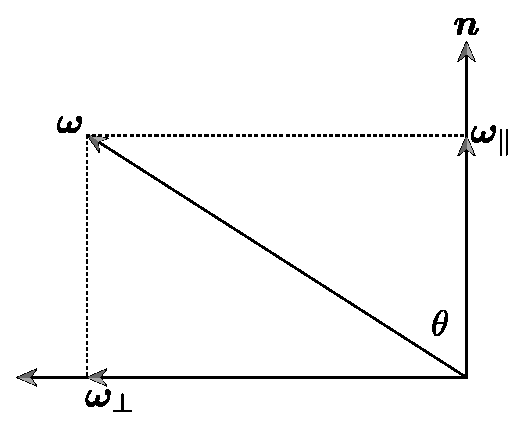
\includegraphics[width=0.4\linewidth]{Pictures/chap08/Parallelprojectionomeganormal.eps}
    \caption{向量$\bm\omega$在法线$\bm n$上的平行投影由${\bm\omega}_{\parallel}=(\cos\theta){\bm n}=({\bm n}\cdot{\bm\omega}){\bm n}$给出。
    垂直分量由${\bm\omega}_{\perp}=(\sin\theta){\bm n}$给出但用${\bm\omega}_{\perp}={\bm\omega}-{\bm\omega}_{\parallel}$计算更简单。}
    \label{fig:8.7}
\end{figure}

\reffig{8.8}展示了计算反射方向${\bm\omega}_{\mathrm{r}}$的设置。
我们可以看到两个向量都有相同的${\bm\omega}_{\parallel}$分量,
且${\bm\omega}_{\mathrm{r}\perp}$的值是${\bm\omega}_{\mathrm{o}\perp}$取反。
因此,我们有
\begin{align}
    \label{eq:8.5}
    {\bm\omega}_{\mathrm{r}}={\bm\omega}_{\mathrm{r}\perp}+{\bm\omega}_{\mathrm{r}\parallel} & =-{\bm\omega}_{\mathrm{o}\perp}+{\bm\omega}_{\mathrm{o}\parallel}\nonumber                                                        \\
                                                                                             & =-({\bm\omega}_{\mathrm{o}}-({\bm n}\cdot{\bm\omega}_{\mathrm{o}}){\bm n})+({\bm n}\cdot{\bm\omega}_{\mathrm{o}}){\bm n}\nonumber \\
                                                                                             & =-{\bm\omega}_{\mathrm{o}}+2({\bm n}\cdot{\bm\omega}_{\mathrm{o}}){\bm n}\, .
\end{align}
\begin{figure}[htbp]
    \centering
    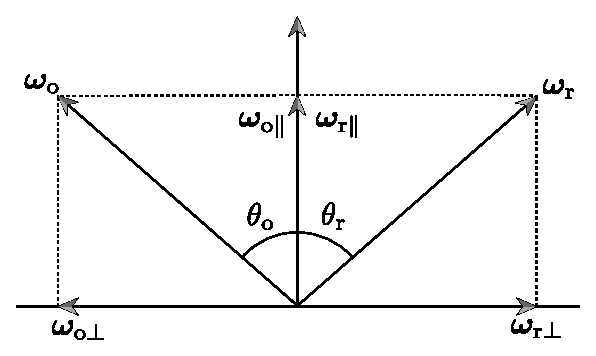
\includegraphics[width=0.5\linewidth]{Pictures/chap08/Perfectreflectioncomponents.eps}
    \caption{因为角$\theta_{\mathrm{o}}$和$\theta_{\mathrm{r}}$相等,
    所以完美反射方向的平行分量${\bm\omega}_{\mathrm{r}\parallel}$和
    入射方向的相同:${\bm\omega}_{\mathrm{r}\parallel}={\bm\omega}_{\mathrm{o}\parallel}$.
    其垂直分量就是入射方向垂直分量取反。}
    \label{fig:8.8}
\end{figure}

函数\refvar{Reflect}{()}实现了该计算。
\begin{lstlisting}
`\refcode{BSDF Inline Functions}{+=}\lastnext{BSDFInlineFunctions}`
inline `\refvar{Vector3f}{}` `\initvar{Reflect}{}`(const `\refvar{Vector3f}{}` &wo, const `\refvar{Vector3f}{}` &n) {
    return -wo + 2 * `\refvar{Dot}{}`(wo, n) * n;
}
\end{lstlisting}

在BRDF坐标系中,${\bm n}=(0,0,1)$,该表达式可极大简化。
\begin{lstlisting}
`\initcode{Compute perfect specular reflection direction}{=}`
*wi = `\refvar{Vector3f}{}`(-wo.x, -wo.y, wo.z);
\end{lstlisting}

\subsection{镜面透射}\label{sub:镜面透射}
\begin{lstlisting}
`\refcode{BSDF Inline Functions}{+=}\lastnext{BSDFInlineFunctions}`
inline bool `\initvar{Refract}{}`(const `\refvar{Vector3f}{}` &wi, const `\refvar{Normal3f}{}` &n, `\refvar{Float}{}` eta,
        `\refvar{Vector3f}{}` *wt) {
    `\refcode{Compute cos $\theta_t$ using Snell's law}{}`
    *wt = eta * -wi + (eta * cosThetaI - cosThetaT) * `\refvar{Vector3f}{}`(n);
    return true;
}
\end{lstlisting}

{\noindent\hfil$=========$\hfil{\color{red}{施工分割线}}\hfil$=========$\
